\documentclass[dvipdfmx,jb5]{jarticle}
\usepackage[top=24truemm,bottom=24truemm,left=20truemm,right=20truemm]{geometry}
\usepackage{amsmath}
\usepackage[]{multicol}
\usepackage{titlesec}
\usepackage{fancyhdr}
\usepackage[dvipdfmx]{graphicx}
\usepackage[dvipdfmx]{color}
\usepackage{color}
\usepackage{url}
\usepackage{ascmac}
\usepackage {fancybox}
\usepackage{jvlisting, listings}
\usepackage[deluxe]{otf}
\usepackage{graphicx}
\usepackage{enumerate}
\usepackage{ulem}

\title{第62回聖光祭 技術部門 引き継ぎ書}
\author{飼沼 隼 \\ 三枝 義啓 \and 浅井 祐一朗 \\ 矢向 俊貴 \and 李 博之 \\ 黒羽 }
\date{2021年 10 月 9 日}

\begin{document}

\begin{center}

\newcommand{\impact}[1]{\textbf{\gtfamily #1}}

\textbf {
\vspace{8.5cm}
\\
\Ovalbox{\fontsize{33pt}{20pt}\selectfont \scalebox{1}[1.2]{超機密}}\\
\fontsize{55pt}{60pt}\selectfont \scalebox{1}[1.1]{技術部門引継書}\\
\fontsize{12pt}{30pt}\selectfont \scalebox{1}[1.1]{聖光祭実行委員会 拡大実行会議}\\
\fontsize{33pt}{35pt}\selectfont \scalebox{1}[1.1]{第1次中間報告}\\
\fontsize{12pt}{25pt}\selectfont \scalebox{1}[1.1]{聖光祭技術部門}\\
\fontsize{12pt}{15pt}\selectfont \scalebox{1}[1.1]{2021年度業務内容概要}\\
\fontsize{12pt}{20pt}\selectfont \scalebox{1}[1.1]{総括篇}\\
}
\end{center}
\pagebreak
\tableofcontents
\clearpage
 \pagestyle{fancy}
\lhead{\fontsize{8pt}{0pt}\selectfont 聖光祭実行委員会\\技術部門引継書 第1次中間報告}
\section{はじめに}
\subsection{挨拶}
こんばんは。第62回聖光祭技術部門長の飼沼隼\footnote{\url{60050kainuma@seiko.ac.jp}}です。この引継ぎ書では業務内容にとどまらず、細かいアドバイスや体験談も交えてできるだけこれ一枚で全てがわかるようにしていくのでぜひ熟読してください。さて、真面目な話は李が下に書いてくれていますので割愛するとして、みなさんには聖光祭を最大限楽しんでもらうべく必要なことを伝えておきたいと思います。一番大切なのは本気でやることです。僕らは初回の会議から一年半準備してきましたが、ずっと死にかけでした。61期の聖光祭は春開催で本当に大変だと思いますが、幹部全員が全速力でやらないと間に合わないですし、やりきった感皆無の聖光祭と青春になることを忠告しておきます。自分がやるだけでは全く足りないです。サボってる人にやらせるのもお互いがやり続けなければだめです。やる作業はひとつだけ、よくできるところを探して直す、これを繰り返すだけです。可能性は無限大です。期待してます!
\\

これをお読みの方、こんにちは。第62回聖光祭技術副部門長の李博之\footnote{\url{60227li@seiko.ac.jp}}といいます。僕が代表してこの挨拶を書かせていただいていますが、もちろん本書はいろんな人が書いています。さて、本書は2021年10月2日〜同4日に開催された第62回聖光祭において技術部門がどのようなことを行なってきたか、そしてその反省をまとめた引き継ぎ書です。技術部門は他の部門と違い、毎回同じことをする部門ではありません。個人のスキルや人材の量と質に大きく作用されます。個人的にはみなさんができる範囲でベストを尽くして欲しいです。僕はこの時の聖光祭でアプリ局長、HP局長、副部門長などを兼任しており、アプリ局iOS班のリードプログラマでした。また、QRコードシステムと統一シフトを個人的に担当していました。忙しいことこの上ないです。そうゆう観点では人事もかなり重要になります。多忙なひとをできるだけ作らないようにしましょう。その人が足を引っ張ることになります。自分語りはこのくらいにしてそろそろ本題に移ろうと思います。この引き継ぎ書がどのくらい続くのかはわかりませんが、後輩の皆さんには絶大な期待と信頼を寄せています。この部門を仲間とともに立ち上げた身としてはできるだけみなさんの後悔がないようにすべてを終え、次に引き継いでもらいたいです。頑張って下さい。
\subsection{本書の取り扱い}
この引き継ぎ書は技術部門及び技術局発足年に書かれたものであり、基本的なことが多く乗っています。ですので、この引き継ぎ書は引き継ぐことをおすすめします。その年々によって修正や改変、追加などがあれば\TeX ファイルを直接編集するか、それを訂正する形で引き継ぎ書を書くのがいいと思います。また、その年あったことを体験談として書くのもいいと思うので別途準備した方が良さそうです。ですが、この引き継ぎ書で全てがわかる状態にするのであればリンクを貼り付けたりするのがいいと思います。
\subsection{Githubと情報公開}
今年から技術部門及び技術局でGithubOrganizationを運営し、全てのコードをGithubで管理することになりました。プログラマにとってコード整理やバージョン管理は重要な課題であり、聖光祭実行委員会と生徒会の透明化のため情報公開は必要だと考えています。Githubの使い方はAPPENDIXにて解説しています。管理者権限等が引き継がれなかった場合、先代の管理者または \url{60227li@seiko.ac.jp}までご連絡ください。
\subsection{開催時期}
今年2021年は新型コロナウイルス感染症(COVID-19)により開催時期は2021年10月2日〜同4日になりました。準備期間が長く、また夏休みを挟んだということを考慮して以下の引き継ぎをお読みください。

\section{基本}
\subsection{組織構成}
\subsubsection{経緯}
2013年、非公式のIT部門が執行部直属に非公式で爆誕。

2014年、外務部門総合技術研究所が誕生。初代所長 綱井先輩\footnote{\url{53127tsunai@seiko.ac.jp}}。

2015年、第二代。少なくとも動画局は存在した。広報委員長\footnote{Twitter: \url{twitter.com/reifujii}}が在籍しており、機材を揃えていたと聞きます。

2016年、第三代。動画作成局とアプリ局の二局が存在した。所長 光藤先輩\footnote{\url{55201mitsudo@seiko.ac.jp}}、動画作成局長は生徒会長の瓜坂先輩\footnote{\url{55031urisaka@seiko.ac.jp}}。

2017年、第四代。この頃の動画局は後者のCGモデル化などを行っていたが、資料は残っていないと思った方がいい。

2018年、第五代。少なくともこの頃には革命が起きていた。傘下に動画局/アプリ局/HP局が存在。総技研は聖光祭の組織だったが、生徒会のサマースクールに際し動画を作るなど、非公式で活動していた。所長兼動画局長 香山先輩\footnote{\url{57084koyama@seiko.ac.jp}. 神。センスと動画のスキルはさることながら、後輩の代になっても差し入れをくれる神。元吹奏楽部Sax}、副所長 新城先輩\footnote{\url{57011araki@seiko.ac.jp}. 神。62回の聖光祭にもいらっしゃった。元コンピュータ部サブチーフ}の二人がピンクT。動画局は香山先輩、新城先輩、平野先輩\footnote{\url{57174hirano@seiko.ac.jp}. 神。社畜で、動画の担当数が異常。元コンピュータ部兼展示団体「総合技術研究所」チーフ} の三人+僕ら60期という感じでした。アプリ局長 [WIP...]

2019年、第六代。58期は前年あまり働いている人がいないのにトップという感じで、カオス。パンフ局はてんてこまいで徹夜続きでした。

2020年、第七代。聖光祭は一般開催では行われなかったが、優秀なエンジニアの所長 沖田先輩\footnote{\url{59039okita@seiko.ac.jp}}や超天才的なスキルとセンスを持ったパンフ局長兼デザイン副課長 柴田先輩\footnote{\url{59091shibataseiko.ac.jp}. 神。元弦オケVc.}など優秀な人材がいた。パンフ副局長兼総技研副所長兼動画局長は飼沼、アプリ局長(ただしみなし幹部)は李、デザイン課長は鈴木瑠之輔\footnote{\url{60111suzuki@seiko.ac.jp}}。

2021年、第八代。部門独立に成功。

\subsubsection{旧組織構成}
(少なくとも2018年)〜2020年の関連する組織構成は以下の通り。
\begin{itemize}
\item 外務部門
  \begin{itemize}
  \item パンフ局
  \item 総合技術研究所
    \begin{enumerate}[−]
    \item 動画局
    \item アプリ局
    \item HP局
    \end{enumerate}
  \end{itemize}
\item 装飾部門
  \begin{itemize}
  \item デザイン課
  \end{itemize}
\end{itemize}

\subsubsection{現在の組織構成}
第62回聖光祭実施時の生徒会技術局、聖光祭技術部門、体育祭技術局\footnote{体育祭のみ、パンフ局・アプリ局・HP局は実質的に存在しない。}の組織構成は以下の通り。\footnote{図括弧内の数字は役職の定数を表す。} \footnote{兼任は妨げていない。} \footnote{生徒会/聖光祭/体育祭でそれぞれ異なったものがある。}\\
なお、名簿はAPPENDIXに記載するので併せて参照のこと。


\vspace{5mm}
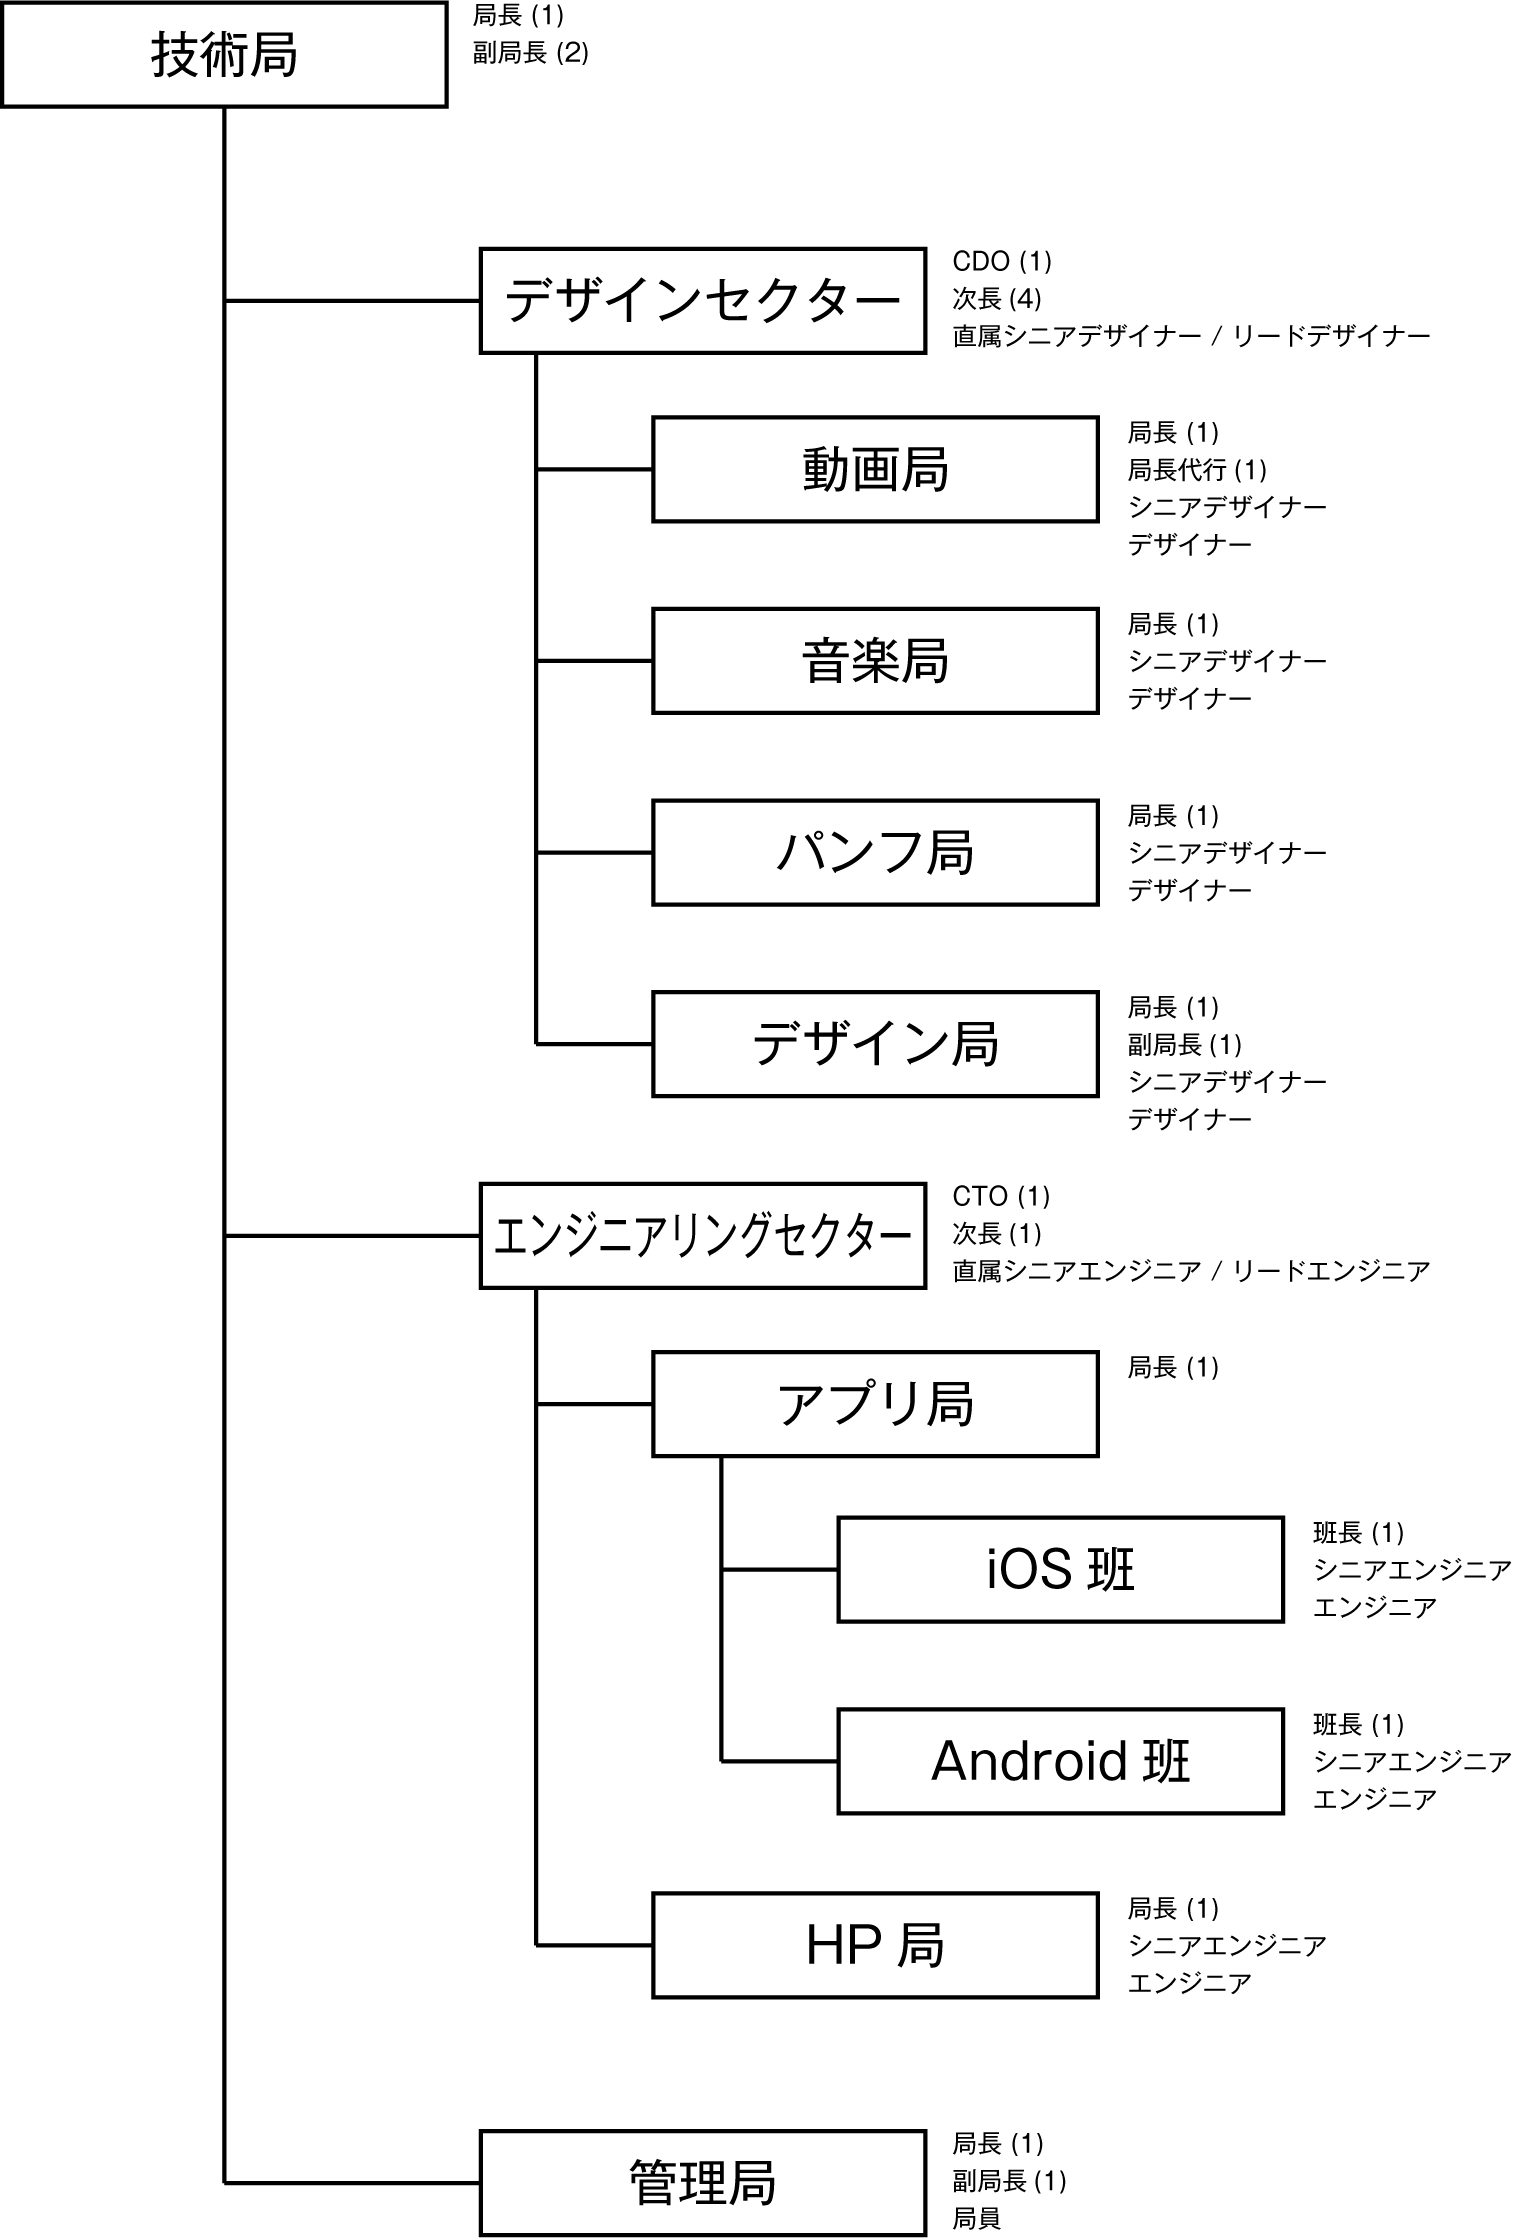
\includegraphics[scale=0.7]{assets/tech.png}\\

\subsubsection{組織}
以下全てにおいて同じですが、上に示した組織形態は60期が決めたものです。君たちがよりよい方法を見つけたらぜひ転換してください。
\begin{itemize}
  \item デザインセクター\\
  内局に4局をもつ。デザインセクターとしては、この4局に振り分けることのできない業務や、この4局に所属しないデザイナーの管理、横断的な業務、デザイン統一等の業務を行う。
  \item エンジニアリングセクター\\
  内局に2局をもつ。エンジニアリングセクターとしては、この2局に振り分けることのできない業務や、この2局に所属しないエンジニアの管理、横断的な業務を行う。特に、統一シフト・QR系のシステム等の開発業務は一切がここに帰属する。
  \item 管理局\\
  名簿作成、書類作成、予算管理、ドライブ(技術局・聖光祭・体育祭・生徒会 etc...)の整理、Slackの整備等の事務(一部技術長・副技術長の事務作業を含む。)を行う。また、技術長・副技術長の事務作業の補佐をする。管理局長の浅井\footnote{60003asai@seiko.ac.jp}が廃止を提言しているので、次期局長の推薦指名は行いません。
  \item 動画局\\
  生徒会、聖光祭、体育祭において、それぞれに関係する各種動画の映像作成・撮影を行う。
  \item 音楽局\\
  動画局の制作する動画の音楽を作るなど、音楽関係の業務を行う。
  \item パンフ局\\
  聖光祭のパンフレットを制作する。生徒会では、DTPデザインを行うこともある。
  \item デザイン局\\
  聖光祭の装飾物のデザインを行う。その他、スローガンロゴのデザイン、アプリ・HP等のUIデザインなども管轄でした(より別のスキルが必要だし、セクターに回してもよい)。生徒会では、選挙広報や外注物のデザインも行っている。パンフ局と協力なりすること。
  \item アプリ局\\
  iOS班とAndroid班に分かれる。それぞれの聖光祭アプリの制作を行う。
  \item HP局\\
  聖光祭HP等の制作を行う。人材不足ですので、次期局長の推薦指名は行いません。次期技術正副部門長推薦内定者で話し合って推薦してください。
\end{itemize}
\subsection{役職と人事、そして自覚}
幹部となったからには、自分の部門の仕事だけしていればいいと思わないでください。全部門の仕事をするつもりでやってください。幹部になるとはそういうことです。人の10倍仕事することを心がけるべし。
\subsubsection{統一}
\begin{itemize}
  \item CDO\\
  デザインセクターの長です。さまざまな分野のデザインに知見がある人で、全体をまとめることができる人がなることが望ましいです。リードデザイナーから一人抜擢すれば良いです。4局に漏れたデザイン業務はここでやります。
  \item デザインセクター直属シニアデザイナー\\
  4局に漏れたデザイナーの局員はここ所属にしましょう。十分スキルとセンスがある人が望ましいです。
  \item リードデザイナー\\
  さまざまな分野のデザインに知見があり仕事ができる人をリードデザイナーとします。大体複数局掛け持ちです。
  \item CTO\\
  エンジニアリングセクターの長です。さまざまな分野のテクノロジーに知見がある人で、全体をまとめることができる人がなることが望ましいです。リードエンジニアから一人抜擢すれば良いです。2局に漏れたシステム業務はここでやります。
  \item リードエンジニア\\
  スキルが高く技術の知見がある人で、仕事ができる人をリードエンジニアとします。大体両局掛け持ちです。
  \item エンジニアリングセクター直属シニアエンジニア\\
  2局に漏れたエンジニアの局員はここ所属にしましょう。十分スキルとセンスがある人が望ましいです。
  \item 各セクターの次長\\
  CDOやCTOに次ぐ人材を入れてください。
  \item デザイナー / エンジニア\\
  各局の局員をデザイナー・エンジニアと呼びます。そのうち技術やセンス、経験が豊富な人をシニアデザイナー・シニアエンジニアとします。
\end{itemize}
\subsubsection{聖光祭}
\begin{itemize}
  \item 技術部門長\\
  拡大実行会議、部門長会議にも出席し、祭全体の梶切りに参加するとともに、それぞれの局の業務を統括します。また実際には、いずれかの(複数の)局の業務を局員として行います。長だからマネージメントに徹して一般スタッフの仕事は行わなくていいというのは大きな間違いです。\footnote{例えば、世界有数の数学の研究所である京都大学数理解析研究所の所長は、歴代フィールズ賞受賞者など、大きな功績を残した数学者が務めています。} 自分自身が貪欲にスキルの勉強をして部門員としても仕事をしてください。また、これは他の幹部も共通ですが、幹部であるという立場として、執行部や他の部門に積極的に切り込んで行って手助けや効率化を行うのは当然です。そして、副部門長をはじめとした多くいる部門幹部に仕事を振り、逆にキャパオーバーぽい幹部(基本全員ですが)を見つけたら程よく手助けするのが肝心な仕事の一つになります。30分睡眠で一ヶ月耐えられる体力とそれでも成績を殺さない学力はつけておくべきです。
 \item 技術副部門長*2\\
  拡大実行会議に出席し、祭全体の梶切りに参加するとともに、担当の局の業務を統括します。青ネク3人それぞれの得意分野を考慮して担当局を振り分けると良いです。また部門長同様、いずれかの(複数の)局の業務を局員として行います。特に今年は、両副部門長とも局長を兼任していました。部門長の補佐をしながら自分の仕事をこなすのは本当に体力がいるので覚悟しましょう。
  \item 各局長などその他の幹部\\
  青ネクではありませんが、拡大実行内でプロジェクトを立ち上げるなど、積極的に祭全体に関わるとともに自分のスキルを最大限活かす方法を考えてください。それぞれの局の業務については他節で記しますので割愛します。
\end{itemize}
\subsubsection{体育祭}
実際の幹部(ピンクT)は以下3人で良いと思います。
\begin{itemize}
  \item 技術局長\\
  週一回から二回の体育祭実行委員会の会議 \footnote{20時半から大体深夜までかかります。} に出席し他の幹部と同様体育祭全体の方針決定に関わるとともに、体育祭全体で技術を使って助けることのできる部分を探していきます。ドライブの管理、名簿の管理、書類の管理などを含みます。当日は運営として走り回ってください。技術部門長と必ずしも同じ人である必要はありませんが \footnote{例えば同じく実行委員会の内局である放送局は放送委員長・放送部門長と異なる人が務めている年「もあります」。} 、まあ長ぐらいは同じでもいいんじゃないでしょうか。
 \item 技術副局長*2\\
  局長とすることはほぼ同じです。当日も走り回ってください。今年は副局長はあんまり会議に来ませんでしたが、できるだけ毎回出席しよう。人事は聖光祭と違くてもいいと思います。
\end{itemize}
\subsubsection{生徒会}
\begin{itemize}
  \item 技術長\\
  技術局の委員会化が公式になされておらず、選挙もしていないので、僕が役員なのかは微妙でしたが、週一回の定例会は毎回でなくとも行くようにしましょう。
\end{itemize}
\subsection{人物}
60期を中心に何をしていた人なのかを逆引きで書いておきます。なお、特記がない場合は生徒会とは第35期生徒会を、聖光祭とは第62回聖光祭を、体育祭とは第36回体育祭を指します。また、特記がない役職は生徒会・聖光祭・体育祭共通の人事です。
\subsubsection{技術}
\begin{itemize}
  \item 飼沼\\
  生徒会技術長。聖光祭技術部門長。体育祭技術局長。CDO、リードデザイナー。シニアデザイナー(デザインセクター、動画局、パンフ局、デザイン局)。動画局長代行。シニアエンジニア(エンジニアリングセクター)。第61回聖光祭総技研副所長・動画局長・パンフ副局長、統一シフトプロジェクトマネージャー。\\
  <略歴>2018/1 外務部門総技研動画局入局。2018/12 装飾部門デザイン課入局。2019/1 外務部門パンフ局入局。2019/5/1 パンフ副局長。2019/5/2 総技研動画局長。2019/5/28 総技研副所長。2020/9 情報技術統括所副所長。
  \item 李\\
  聖光祭技術副部門長。体育祭技術副局長。生徒会監査副委員長(DX)。CTO、リードエンジニア。シニアエンジニア(エンジニアリングセクター、アプリ局iOS班、Android班、HP局)。HP局長。シニアデザイナー(デザインセクター;UI)。アプリ局iOS班長。第61回アプリ局長、聖光祭統一シフトリードエンジニア。\\
  <略歴>2018/1 外務部門総技研アプリ局入局。2019/5/2 総技研アプリ局長。
  \item 浅井\\
  生徒会副技術長。聖光祭技術副部門長。体育祭技術副局長。リードデザイナー。シニアデザイナー(デザインセクター、動画局、パンフ局、デザイン局)。管理局長。
  \item 鈴木\\
  生徒会デザイン局長。聖光祭装飾副部門長、デザイン副局長。体育祭デザイン局長。デザインセクター次長、リードデザイナー。シニアデザイナー(デザインセクター、動画局、デザイン局)。\\
  <略歴>2019/3 装飾部門デザイン課入局。2019/7 外務部門総技研動画局入局。
  \item 黒羽\\
  デザインセクター次長、リードデザイナー。シニアデザイナー(デザインセクター、パンフ局、デザイン局)。パンフ局長。\\
  <略歴>2019/5 外務部門パンフ局・装飾部門デザイン課入局。
  \item 三枝\\
  デザインセクター次長、リードデザイナー。シニアデザイナー(デザインセクター、動画局、パンフ局)。動画局長。シニアエンジニア(エンジニアリングセクター、アプリ局iOS班)。\\
  <略歴>2018/3 外務部門総技研動画局入局。
  \item 満田\\
  シニアデザイナー(音楽局)。音楽局長。\\
  <略歴>2019/1 外務部門総技研動画局入局。
  \item 矢向\\
  シニアエンジニア(エンジニアリングセクター、アプリ局Android班)。アプリ局長。
  \item 鬼頭\\
  シニアデザイナー(デザインセクター;CG)。シニアエンジニア(エンジニアリングセクター、アプリ局Android班)。
\end{itemize}
\subsubsection{その他}
\begin{itemize}
  \item 大下\\
  聖光祭実行委員長。シニアデザイナー(パンフ局、デザイン局)。管理局員。第61回聖光祭副実行委員長。
  \item 古澤\\
  聖光祭副実行委員長。シニアデザイナー(パンフ局)。
  ...
\end{itemize}
\subsection{教職員}
関係する教職員を逆引きで示す。以下は全て2021年度のもの。学校は会社同様、年度で人事も全て刷新される(変更がある可能性も大いにある)。
\subsubsection{事務}
\begin{itemize}
  \item 事務室\\
  \item 野口先生\\
  事務長。
\end{itemize}
\subsubsection{教員}
情熱がある先生、生徒を大事にしてくれる先生がほとんどですが、それでも大人。教職も忙しいですし、面倒なことは断られやすいです。その上でどう通すかを考えよう。
\begin{itemize}
  \item 職員会議\\
  職員の会議は木曜日(多分)。また、毎朝8:10〜朝礼で教務主任の小泉先生が全先生に連絡事項を伝達します。HRでの伝達は担当先生経由で小泉先生にお願いしよう。ちゃんと聞いてない先生や忘れる先生もいるので、その誤差に注意。

  \item 生徒指導部\\
  飯岡先生、石渡先生、滝本先生、川部先生、等々がいることしかわかりませんが、企画書等はここで審議されます。急ぎのものがあっても、生徒指導部の会議は金曜(変更になっている可能性があるので先生に確認のこと、4月では多分変わります)4限で固定なので、これを待たなければいけません。

  \item 飯岡 雄介 先生\\
  聖光祭顧問。執行部顧問。理科科(化学)。S3D担任。バレー部顧問。少し厳つい先生ですが、だいたい優しいです。キレると少し怖いです。

  62回では高3の担任をしながら聖光祭の顧問をやるという過労。飯岡先生のやることは超多いので、迷惑や心配をかけないように。飯岡先生と仲良くなると色々うまく回ります。部門顧問をかっ飛ばして飯岡先生に相談するのも度を過ぎなければよいです。早寝早起きです。月曜研修。

  \item 石渡 巧 先生\\
  生徒会顧問。執行部顧問。社会科(世界史)。S3C担任。陸上部主任顧問。だいたい優しいですが、問題発言をする癖があります。本人のいないところで陰口を行ったり、僕が欠席した予算審議で技術局の悪口を言ったりしてました。

  それと、基本的に全てを忘れています。自分で決済した物品も1週間後には何も覚えていません。それを考慮して動かないとひどい目に遭います。石渡先生も忙しい方ですので、早めに相談しよう。木曜研修。

  \item 川部 大輔 先生\\
  体育祭顧問。聖光祭企画/演出顧問。体育科。S1E副担任。バレー部主任顧問。面倒です。基本は優しいですが、生徒を小馬鹿にしています。一度話し始めると長いです。話すのは最小限にすべく、川部先生の追及を受けることがないようにしよう。ブチギレると体罰もします。土曜研修。

  \item 宇佐美 直也 先生\\
  聖光祭技術顧問。理科科(生物)。S2D副担任。生物部主任顧問。
  \item 山口 ゆり 先生\\
  情報科。
  \item 河野 周 先生\\
  英語科。S2B担任。硬式テニス部顧問。
  \item 百武 沙紀 先生\\
  英語科(帰国英語)。
  \item 神保 元 先生\\
  国語科(現在は古典)。J2C副担任。コンピュータ部主任顧問。
  \item 小泉 直範 先生\\
  教務主任。数学科。
  \item 花家 徹 先生\\
  副校長。社会科(現代社会家庭、現在は特別科目のみ)。
  \item 滝本 先生\\
  \item 松原 先生\\
  \item 出口 先生\\
  ...
  \item 工藤 誠一 先生\\
  校長。社会科(政治経済公民、現在は教職なし)。
\end{itemize}

\subsection{立場と名称}
\subsubsection{生徒会}
59期の齋藤先輩が「情報技術統括所」(略称:「ITEC」)という謎名称をつけてしまったところ、「総合技術研究所」「技術局」の名前と混乱され多分俺らしかわかってない。近い人には「情技統」「情統」「ITEC」の名前で呼ばれる。僕(飼沼)はGTECっぽくてあんまり好きじゃないので、「技術局」(役職の場合は「正副技術長」)を使いがちです。第35期生徒会役員会において委員会化が全会一致で可決し、オンライン投票の試験運用として委員会化の全校投票および首長の選挙が行われる予定であったが、スケジュールが合わず不可能となった。委員会化は可決しているので、次年度も役員会で過半数(賛否同数の場合は生徒会長の決定による)の反対がない場合は、委員会化投票の手続きを進めても問題ないであろう。「技術局」は事務局・会計局と混同される恐れ、「技術委員会」は怪しそう、等々の意見があったので、次年度の解決に委ねます。
\subsubsection{聖光祭}
第62回聖光祭にて部門独立。飯岡先生に大下から無理を言って幹部の人数を申請したので、これ以上増やすとなるとさらに交渉が必要か。基本的に教員に煙たがれていることを理解し、お取り潰しなどないよう、{\bf 期限などは絶対守るように行動}すること。
\subsubsection{体育祭}
第35回体育祭にて技術課として設置。第36回体育祭にて技術局(放送局・新設の装飾局とともに実行委員会内局)となる。

\subsection{予算}\label{sec:予算}
\subsection{ハード機材引継}
\subsubsection{動画局管轄}
 現在動画局(生徒会)で所有している機材は以下の通りである。
 \begin{itemize}
  \item BlackmagicDesign Pocket Cinema Camera 4K\\
  広報委員会が生徒会予算で購入している。
  \item DJI RSC2\\
  カメラ用ジンバル。動画のプロジェクトで必要な機材として、工藤校長先生に購入していただいた。
  \item グリーンバック\\
  使おうと思って購入したが、結局使っていない。ぜひ使って欲しい。
  \item Windows Desktop PC (自作)\\
 40万くらいかけて自作したPC。CGのレンダリングに最適。
  \item Square\\
  9台ある。
 \end{itemize}

 \subsubsection{学校管轄}
 学校側が所有しているが我々が使用できる機材。
 \begin{itemize}
  \item iPad (第八世代)\\
  20台を学校が所有している。\\
  使用する際は情報科の山口ゆり先生\footnote{\url{yuri.yamaguchi@seiko.ac.jp}}に頼むこと。
  \item RODE Wireless Go\UTF{2161}\\
  ワイヤレスマイク。送信機二つと、受信機一つ、3.5mmイヤホンジャックケーブルが含まれる。使用する際は事務局長の野口先生\footnote{\url{noguchi@seiko.ac.jp}}まであらかじめメールで連絡し、事務室に取りに行くこと。返却する際もあらかじめメールが必要。
 \end{itemize}

 \subsection{ソフト引継}
 \subsubsection{メアド}


\section{概括}
\subsection{スケジュール}
\subsubsection{選挙まで}
任命式までは幹部としての資格はないことに注意。ただ拡大実行など会議は積極的にやったほうがいいと思います(62回の場合は 2020/5 第一回拡大実行、9 第二回拡大実行、 11 第三回拡大実行、 12初旬 規則関係会議、12中旬 第四回拡大実行 など)。引き継ぎが死ぬほど大変だったので、この頃から毎日日記を書いてると楽かも。

\subsubsection{選挙あと}
幹部名簿は作り始めましょう。こういうのは技術が先導してください。実行委員長が後に飯岡先生から提出用のシートを渡されるので、青ネクのみとピンクTまでを両方作るべきかと思います。学年/クラス/出席番号/学籍番号/メール(以上は統合名簿からvlookupでどうにかできます)/誕生日(ふりふら登録用)/掛け持ち予定 を記録しよう。

\subsubsection{副実行委員長面接}
実行委員長を助けてください。募集の資料を作成し、Classroomで中3/高1に配信。高2副を決めた後、高2副全員で高1副の面接。多少の助言はありだと思います。副実行委員長が誰かは本当に大切です。君らの命綱です。また、{\bf \ref{sec:議事録班}} にも書きますが、面接の発言録をとってください。

\subsubsection{初回オフライン拡大実行}
幹部が全員確定した時点で拡大実行を行って全員で顔合わせをしよう。ふりふらの団体登録(もうしてあるかな?)を済ませ、全員でLINEスケジュールなどで予定調整し一研を早めに予約しよう。初回ではお世話になるふりふらの方を呼び入れて全員で挨拶すること。反省点の洗い出しと新しくやりたい企画などについて話すといいと思います。

\subsubsection{任命式}
毎年、2学期期末試験最終日に飯岡先生から聖光祭幹部に聖光祭活動に当たっての諸注意があります。この任命式を以て、内定している聖光祭幹部が学校側として正式に認められることになります。この日以降は、聖光祭活動が正式に認められます。任命式終了後は幹部全員で顧問教諭に挨拶しにいきましょう。

\subsubsection{冬休み}
冬休みは全て聖光祭に捧げるくらいでいきましょう。執行部に確認し、活動予定表を埋める必要があれば期限厳守で提出すること。特に撮影などをしたい場合は顧問教諭と飯岡先生両方に確認を取りましょう。また、全部門で倉庫(41等)の整理をするといいと思います。管轄を決め物品を全てスプレッドシートに書き出しましょう。

\subsubsection{部門ガイダンス}
1月に行われる部門ガイダンスの資料作成をしてください。冬休み明けにすぐに先生方の校閲を受け、生徒会室の画鋲を使って幹部全員で協力して各教室の後ろにガイダンス資料を貼りましょう。中学1年生を放課後小講堂に集めて各部門長から各部門の紹介をします。紹介するためのスライド、手元でも各部門の仕事が確認できるよう部門ガイダンス資料を作成しておこう。スライド原案は各部門が作りますが、デザイン統一は技術がやってください。発表する際は、腕章を忘れずに、身なりも整えてくること。印刷は聖光祭執行部経由で頼みましょう。

\subsubsection{部門動向調査}


\subsubsection{第一次予算審議}
{\bf \ref{sec:予算}} を参照。



\subsection{各部門との連携}
聖光祭で大事なのは幹部間の情報共有です。お互いに何の仕事をしているのか共有し、開放感のある雰囲気を作り、拡大実行全体で一体となって行動しよう。さもなくば聖光祭は失敗します。

\subsubsection{執行部}
執行部は全てを取りまとめるところ。だからこそ、失敗を怒られもするし、逆にサボっていたら怒るのが正しいです。ただ、執行部は本当に忙しいです。時に部門の仕事をたっぷり肩代わりしたり、相当な責任を背負っていたりします。感謝と思いやりを持って接し、仲良くしよう。

執行部はやることが漠然と(「サポート」「取りまとめ」)していますし、タスクが積み重なっている忙しい部署ので、執行部全体に頼んでもヘルプが帰ってこないのは茶飯事です。こちら側から直接メンションし、「担当は〜でいい?」「〜までに〜をやるのを手伝って欲しい」とお願いしよう。どんなに忙しくてもコミュニケーションをサボるのはだめです。

何かあったらすぐに執行部に相談しよう。執行部と相談して進めるのが一番大事です。また、執行部が死にそうな時は、積極的に仕事を手伝おう。技術部門の鉄則:「自分が執行部であるかのように行動しよう。」

飯岡先生や石渡先生と話がしたい時は、執行部に仲介してもらうか、一緒に職員室に伺うのがよいです。

\subsubsection{演出部門}\label{sec:演出部門}
演出部門はバンドを統括するところ。一方で、グラフィナなどの舞台演出の仕事を企画部門とともに担当します。ですから、動画局・音楽局は積極的に演出とコンタクトを取りましょう。講堂関係なども、全体でコンセンサスが取れている状態で教員と交渉しよう。\\
{\bf 注} バンド掛け持ち幹部の演出の所属有無について決めておこう。後々名簿に追加する事になると面倒です。

\subsubsection{外務部門}
外務部門は対外関係全てを統括するところ。入場関係のシステムでは外務ときちんと調整しよう。

また、ポスターとパンフの入稿関連の管轄を事前に決めてください。パンフの広告は外務が担当しますが、ポスター・パンフの入稿作業は執行部がやるのか?技術がやるのか?外務がやるのか?仕事の忙しさによっては管轄を変更しよう。外務は細々とした作業がずっとあります。連絡が遅くなると本当に迷惑をかけますので、注意してね。

送付状の差込についてはGASで自動化してあげてください。{\bf \ref{sec:外務送付状の差込}} 参照。

\subsubsection{装飾部門}


\subsubsection{企画部門}


\subsubsection{食品部門}


\subsubsection{放送部門}


\subsubsection{美化部門}


\subsubsection{展示部門}


\subsubsection{会計部門}


\subsubsection{管理部門}

\section{動画局}
\subsection{ソフト}
 動画を作る上で必要なアプリケーションを紹介しておく。
 \begin{itemize}
  \item Adobe系\\
  学校から支給されているものを使えば良いと思う。
  \item Davinci Resolve Studio\\
  BBMPCC 4Kを購入した際についてきたものが、生徒会室のPCに割り当てられている。普通に買うと3万円くらいする。カラーグレーディングに最適。
  \item Cinema 4D\\
  CGソフト。40万くらいする映画にも使われているソフトだが、学生は実質無料\footnote{別の会社のプラットフォームを使って購入するため数百円の手数料が取られる}で使える。
  \item Octane\\
  レンダラー。Cinema 4Dと共に使うととてもいい映像が出来上がる。
  有料であるが、予算で落として使うべし。\\ただし、1,2アカウントを何人かで使うことになり、同時に使用することができないので注意が必要。\\生徒会室のPCをレンダリング専用に割り当てたいので、2アカウント購入すべし。
 \end{itemize}
\subsection{動画}
最低限作るべき動画は以下の通り。
 \begin{itemize}
  \item スローガン動画\\
  フルCG。聖光祭関連の最初の動画となるので、聖光祭二ヶ月前から一ヶ月程度で完成させるべし。
  \item 幹部紹介動画\\
  第62回聖光祭では、各部門に演出を考えてもらって三学期期末試験最終日後と終業式後に撮影した。とても大変だったが好評だった。61回以前では各部門の集合写真にテロップをつけたもので生徒総会で流しても寝てしまう人が多かった。

  \item オープニング動画\\
  聖光祭一日目の開会式で流す映像。内部向け。
  \item グランドフィナーレオープニング動画\\
  聖光祭最終日のグランドフィナーレで流す映像。外部向けなので技術力を見せつけるチャンス。
  \item エンディング動画\\
  聖光祭片付け日の閉会式で流す映像。聖光祭期間中に撮影された写真のスライドショー。
 \end{itemize}


  \section{HP局}
 62回局長:李博之(60227)
 \subsection{ソフト}
 あくまで僕が使用したソフトである。htmlとcssとjsをいじれるならなんだっていい。
  \begin{itemize}
  \item Visual Studio Code\\
  エディタ。自分好みに機能やデザインをカスタムできるため、汎用性が高い。Microsoft社製でもちろん無料。同じようなものでGitHubが出してるAtomというものもあり、個人的にはAtomの方がデザインはいいと思う。VSCodeにAtomizeというプラグインを入れてAtom風にしていた。プラグインは後ほどまとめる。
  \item Adobe XD\\
  UI/UX設計ソフト。他のAdobeソフトとの互換性がとてもいい配置ソフト。オブジェクトを配置してサイトのUIを検討することができる。直感的に操作でき、画面遷移もシュミレートできる。ただし、CSSやHTMLを書き出してくれるわけではないので必須ではない。個人的には仮でもUIのイメージがあると作りやすいので必ず使っている。
  \item Adobe Dreamweaver\\
  ウェブアプリ制作の統合型開発環境的なもの。初期段階で使うことを検討していた。ウェブ制作のすべてがここにある。リアルタイムのUIシュミレートやサーバーへの更新設定、サイトの公開もやってくれる神ソフトだが、重いのが難点。パソコンを変えたときにインストールを忘れていて自然消滅した。正直全く不満はなかった。
  \item その他Adobeソフト\\
  デザイン局が忙しそうだったので素材は全部自分で作った。楽しい。Illustratorは使えないと恥ずかしい。
  \item FileZilla\\
  いわゆるFTPクライアントソフトというもの。FTPサーバーにファイルをアップロードするときに使う。FFFTPとか有名どころは他にもある。すべてUIが古いWindows感でてて怪しいが全然普通のソフト。FTPについては後ほど解説する。
  \item Firefox Developer Edition\\
  ブラウザ。Chromeでブラウザアカウントを学校アカウントにしてると開発者モードが使えないのでこれを入れた。Developer Editionのとおり、開発者に嬉しい機能が割とある。Chromiumで動いているので環境はあまり変わらないはず。
 \end{itemize}
 \subsection{フレームワーク}
 僕が使用したフレームワーク。
  \begin{itemize}
 \item nuxt.js\\
 サイトが作りやすくなるフレームワーク。流行ってるので使った。必須ではないかな。
 \item firebase\\
 サイトをホスティングするのに使った。詳しくは体験談を読むこと。
 \end{itemize}

 \subsection{スケジュール}
 \begin{itemize}
 \item ベースデザインの確立(1週間)\\
 デザインを設計する上で大切なのは指向となるベースデザインだ。例えばモノクロでいくのか、パステルカラーを使ったハイトーンでいくのか、はたまた原色よりの複雑なデザインにするのか。文面や口で説明するのは非常に難しいがPinterestを使うといい。Pinterestは自分が気に入ったアイディアを保存でき、その傾向によってまたタイムラインを更新してくれるというもので使い方などは各自で調べて欲しい。これを利用することで自分の好きなデザインを集めて考えることができる。スローガンになるべくあったものを探すべきだが自分の場合、これが好きだとおもったデザインに後ほど意味づけを行なった。意味づけとはデザインのオブジェクト一つ一つに意味を持たせることである。この作業は単に意味を頭の中でつけるのではなく、実際にオブジェクトをつけた意味に近いものに修正しながら行う。これをみた1人でもいいからこの意味に気づいて欲しいと思いながらやる。実際はだれもわからないものでもその意味づけの改変がデザインをより良いものとしていく。
 \item オブジェクトの配置(1週間未満)\\
 ベースデザインが決まれば次は実際に作ってみる。紙でもPC上でもホワイトボードや黒板でもいい。一回それを簡単な方法で表現してみる。自分はスケッチブックに一回書いて修正し、ある程度できたら今度はAdobe XDで表現し、また修正するというプロセスを踏んだ。いきなりソースコードを書くと一つのオブジェクトを配置するのに時間がかかる上、修正の小回りが効かない。説明する順番は逆になったがこれが終わったら先述した意味づけを行う。
 \item 環境の構築(1日〜数日)\\
 ローカルにプロジェクトをつくって環境を整える。併せてFirstCommitをしてRemote RepositoryにPushする。
  \item ホームの制作(2週間)\\
  長い時間をかけていいので緻密に作る。載せる内容はトップ\footnote{開いたときに表示されるやつ}、お知らせ\footnote{告知のなかから抜粋}、スローガン\footnote{スローガン動画公開まで非表示}、実行委員長から\footnote{ポエム}、フッター、サイトマップやメニュー。他は自由に追加して構わない。
  \item サイトの公開\\
  聖光祭開催1ヶ月前を目安に公開する。その後、SNSや学校のサイトで宣伝する。個人的には1ヶ月前だと遅い気すらする。
  公開には時間がかかるため、SNSや学校のサイトで告知される前にはもう公開しちゃおう。(どうせ調べても出てこない)その際、しっかりSEO対策\footnote{SEO対策とはGoogleなどの検索エンジンロボットにサイトの内容をより正確に取得してもらうようにすることを指す。}をする。僕はサボっててサイトの説明文すら書いてなかったが途中で気づいて書いた。サイトの公開後はGoogleSearchConsoleにサイトを登録。Google検索で自分のサイトがどれくらい検索されてて掲載順位がどのくらいなのかをみることができる。GoogleRobotがどのくらい来たかもみれる。登録にはサイトの所有者を証明する必要があるため、Googleからもらったhtmlを直下に置いたり、metaタグを追加したりする。所有者が証明できたらとりあえず安心できると思う。3日後ぐらいまでには記録が開始され、掲載順位や訪問者数のグラフが表示されるだろう。
  \item サイトの運営\\
  聖光生や暇な先生って結構優秀で間違いやバグを報告してくる。その報告を治しながら次は他のサイトの制作を始める。
  \item サイトの順次更新\\
  情報がUpdateされるごとにサイトを更新していく。展示団体が確定すれば展示団体一覧を、食品店舗が確定すれば一覧を、校内Mapやスローガン、余裕あれば取材などして記事を投稿するのもいいだろう。ある程度自由にできるので楽しもう。
 \end{itemize}
 \subsection{ウェブサイトを作る上での基本知識}
 余計なお世話かもしれないが、最低でも以下のことは覚えとこう。
 \subsubsection{リクエストとレスポンス}
 端末からサーバーへの問い合わせ(Request)とそれに対する応答(Response)の関係は何があっても覆すことはできない。Requestなしにサーバーがいきなり端末に通信をすることはできないのである。
 \subsubsection{サーバーという概念とURL}
 我々が使うのはおもにファイルサーバーというものである。他にアプリサーバーやDBサーバーが存在する。URLはサーバーに存在する全てのアクセス可能なファイルに対して与えられ、パスと同義である。URLのオーソリティはサーバーを特定しその後は設定したルートファイルからの相対パスになっている。オーソリティはプロトコル、サーバー名、ドメインでできている。例えばPC名www、ドメインseiko.ac.jp内のroot/2021/articles.htmlのファイルのURLはhttps://www.seiko.ac.jp/2021/articleとなる。プロトコルとドメインは次項で解説する。
\subsubsection{プロトコル}
プロトコルとはある通信が何についてのどんな形の通信なのかを表す規定された文字列のことである。当然この世界にはWebサイト以外の通信もあり、物理層、データリンク層、ネットワーク層、トランスポート層、セッション層、プレゼンテーション層、アプリケーション層の7層でできている。下の層になるほど物理的で単調な信号になる。これはあくまでプロトコルの分類の概念である。ちなみにこの概念はOSI参照モデルといって現在はTCP/IPという別の概念が使われている。端的に言えば「何を送るのか」を表しているのである。例えばHTTPはウェブサイト、HTTPSは暗号化されたウェブサイト、SMTPはメールの送信、POPやIMAPはメール受信\footnote{厳密には移動とコピーの違いあり}、FTPはファイルやフォルダーの送信などがある。アクセスしたファイルをどんな形で取ってくるのかを表し、ブラウザがレンダリングするときに使われる。
\subsubsection{ドメインとサイト取得までの流れ}
今回は作りたての学校のHP http://www.seiko.ac.jp/ に自宅にあるPCから始めてアクセスした時を考えてみる。\footnote{なんでhttpなんだよ...} まず、URLを叩く。その通信は無線LANで繋がっているルーターから自宅地下の電話線を通り近くのキャリア基地局までくる。データセンタとも呼ばれるところである。\footnote{Googleデータセンタなどのデータセンタとは別物}URLはネットの住所ではないのでURLだけで直接どこかにアクセスことはできない。使用するのはIPアドレスであり、とりあえず聖光HPのIPアドレスを探したい。ここで一度基地局内のキャッシュサーバを通しキャッシュから探す。以降のキャッシュサーバでも同じだが今回はサイトも端末も新しいのでキャッシュにはないとする。キャッシュサーバ通したときにあればそこで折り返されると考えて良い。今回はキャッシュにないので権威DNSサーバにアクセスする。ドメインは逆側から読む\footnote{今気づいたけど外国の住所と同じやな}のでjp\textgreater\textbar ac\textgreater\textbar seikoという構造である。権威DNSはjpノードに案内し、jpノードはsc(教育機関)ノードに案内する。そしてscノードにはseikoという名前のサーバのIPが登録してありこれを取得するという形でURLとIPの交換が完了した。ドメインは入れ子構造になっていて逆から読むということは覚えとくべき。もらったIPを使えば簡単に聖光のルータにアクセスできる。ルータからPC名(今回はwww)を渡すことでパソコン内のルートフォルダにアクセスする。パスには今回何も書かれてないが/で終わることは暗示的にindex.htmlを指すことが設定されてるはず\footnote{場合によってdefault.htmlなど、サーバ側の設定で変えることはできる}なのでindex.htmlを取得し端末に帰っていく。
\subsubsection{サイトのレンダリング}
HTTP通信のうち、サイトのhtmlを取得したりする\footnote{一般化するとdoGet()をコールするということだが}ことをGET通信と呼ぶ。これに対して、サーバに対して情報を渡すときに使うのがPOST通信である。先述したindex.htmlをGETするのが第1ステップになっており、そのhtmlを取得したブラウザは\verb|<head>|タグを読む。そこには\verb|<link>|タグや \verb|<script>|タグでcssやjsが紐づけられており、今度はこのcssやjsをGETしにいく。その間に\verb|<body>|タグ内を読み、\verb|<img>|タグや\verb|<video>|タグ、\verb|<iframe>|タグなどのリソースを取りに行く。また、読み込んだ\verb|<body>| タグ内のオブジェクトを描画し、cssをもとに再描画。\footnote{この間僅かなので見えない。ネットが遅いと見れる。}最後に\verb|<img>|タグや\verb|<video>|タグ、\verb|<iframe>|タグなどのリソースが届き、当てはめる。javascriptが実行され、すべての作業は終了する。以上を見るに何回もGETを繰り返してるのがわかる。これは開発者モードで見ることができる。
\subsubsection{FTPクライアントの使い方}
FTPサーバにファイルを送信したり取得するときは「FTPユーザ名」と「FTPパスワード」と「FTPホスト」が必要である。「FTPユーザ名」はドメインと同じなのでseikofes.official.jp。また、FTPホストはsv64.star.ne.jp。この三つは一緒にITEC長のパスワード一覧的なものに掲載してもらってる(はず)なので、部門長に問い合わせてみること。FTPクライアントに少し名称は違うかもしれないが、この三つを入力する。あとは接続ボタンを押せばOK。僕が使ったFileZillaは左側にローカルのファイルツリー、右側はFTPサーバのファイルツリーが表示されており、ドラッグ\&ドロップでファイルを移動できるようになっていた。また、Starserverの方からもアクセスでき、ファイルのアップロードはできないが確認としては役立つだろう。
 \subsection{反省点\&注意次項}
 \subsubsection{顧問挨拶}
 部門の顧問の生成と挨拶するときにかならず「starserverの代金は払っているかの確認」をしてもらうようにすること。今年2021年、3人の先生に確認して「払っている」と言われていたが結局、支払い催促メールが届いていた seikofesta@gmail.com を誰も見ておらず、契約解除となってしまった。(もともとは seikofesta.official.jp だったと記憶している)seikofesta@gmail.com にアクセスできる唯一の先生が夏季休暇のため音信不通になってしまったのも起因してしまった。夏休み中は先生と連絡できるとは限らないのでもし、聖光祭の開催時期が2学期だった場合、注意が必要である。
 \subsubsection{時間を作ろう}
 基本的にHPの仕事がメインだと思うが自分の場合はそうではなかった。むしろ副業みたいなものだったので時間はあまり作れなかった。これによってHPは中途半端なところで終わってしまった。食品店舗は終了したのでCOMING SOONを表示してると思うが、マップや記事ページは終わってない。記事は投稿できる仕組みを作ったが、Firebase Realtime Databaseにデータ入力する必要があり時間がなくてほとんど投稿できなかった。これは猛省している。麻布(2020?)ではアカウント制にしており、幹部などが自由に書き込みできる。(自分の代はそうゆうのを逆手にとっていたずらする問題児がいたのでどちらにしろ実現できなかったが)その代の風紀を鑑みた上、人を絞るあるいは記事投稿班を作るなどしてやってみるのも面白いと思う。灘(2019)ではMarkdown記法をHTMLに変換するライブラリを使っていた。いちいちサイトを更新しなければいけないがいい考えである。\footnote{2019灘の文化祭「SAIL AWAY」のHPは高校生が作ったと思えない神サイトである。ぜひ一度見て欲しい。}
 \subsubsection{仕事を整理しよう}
 HP制作中は素材関連の連絡や修正の申し出、仕様変更の申し出などが多くあり、HPに掲載する情報を整理するだけで一苦労である。付箋を使ったタスクの管理は古いと思われがちだが、あれはすごい効果的だ。自分は自分の席が壁列だったので壁に付箋を貼っていた。それによって仕事が捗ったのは事実だ。PC上で管理できるが結局は開くのがめんどくさい、タスクの登録がめんどくさいなどで逆効果だった。ぜひ取り入れて欲しい。

 \newpage
 \section{アプリ局(Android)}
 \subsection{はじめに}
 引継書とは題しているがAndroid作る人は全員読んでおいて損はないのではないかと思われる(今年出してもらったプログラムの出来栄えを見る限り)。\par
かなりメモっぽく書いているので注意。Discordで皆に連絡
するときの感覚で書いていると思ってもらえると内容が入りやすいかもしれない。
 \subsection{技術幹部になった人へ}
 個人的に技術幹部となった人に要求されることは高い技術力よりも\mark{仕事をミス無く丁寧に確実にこなすこと}なので注意(もちろん自分の担当する分野においてある程度の知識は持っていなければいけないけれど)。技術力があったとしても、
 \begin{itemize}
 \item 提出期限を守らない
 \item ミスが多い
 \item 連絡ができない
 \end{itemize}
 といった人は技術幹部に限った話ではないけれどお仕事にならなかったり、もしくは周りに迷惑を書けてしまい他の幹部に陰口を叩かれてしまったりする(後者はよく見た気がする)。\par
くれぐれも技術力があるからといって他の部門の幹部などに対して調子に乗った言動をしたり高圧的になったりすることがないように(まぁこんなことはほぼなかったと思うけど)。
 \subsection{全体として}
  \subsubsection{制作の前準備}
 今回なら聖光祭は9月で、UIなどの案が挙がってくるのが8月であったけれど、アプリの試作自体は5月から始めていた。\par
 特に自分に作ることができるか不安な箇所を中心に自分で事前に試作をしておくとよい。
 矢向なら
 \begin{itemize}
  \item RecyclerViewの使い方
  \item RecyclerViewを横に2つ、それを縦につなげていく方法
  \item HTTP通信
  \item Fragmentを画面に一部に収める(全画面に出さない)
  \item DBの使い方
  \item アプリアイコンの設定法
 \end{itemize}
 など
 \subsubsection{実装方法の基本方針}
 同じ挙動にもいくつかの実装方法が当然考えられるわけだが、どの方法を使うかを選ぶときに重要なことを重要度順にあげていく。
 \begin{enumerate}[No.1]
  \item エラーが起こりづらいこと(起こらないこと)
  \item 動作が軽いこと(=ユーザーが快適に使えること
  \item コードが読みやすいこと(=保守性が高いこと)
  \item 実装方法がオシャレであること
 \end{enumerate}
1と2は最優先事項。とくに1。カッコつけて新しいライブラリを使ってエラーが起こりました、ではお話にならない。また、この4点はお互いに関係があり、1つを守ることが他の2つを守ることにつながっていくので常に頭に入れておきたい。
 \begin{itembox}[l]{余談}
 現在唯一人間を国際宇宙ステーションへ輸送することができるロシアの有人宇宙飛行船「ソユーズ」では、動作環境が宇宙空間であるために事故は絶対に起こってはならず、そのためソユーズを制御するコンピューターにはあえて新しいものではなく、動作が保証されたかなり旧式のものが使われてるそう(ソユーズに限った話ではないけれど)。つまるところアプリ開発においても古いライブラリなどを使えとは言わないけれど(というかむしろ古すぎると逆にエラーが起きることが多い)プログラムの安定性を最優先にしましょうということ。\par
 \begin{center}
 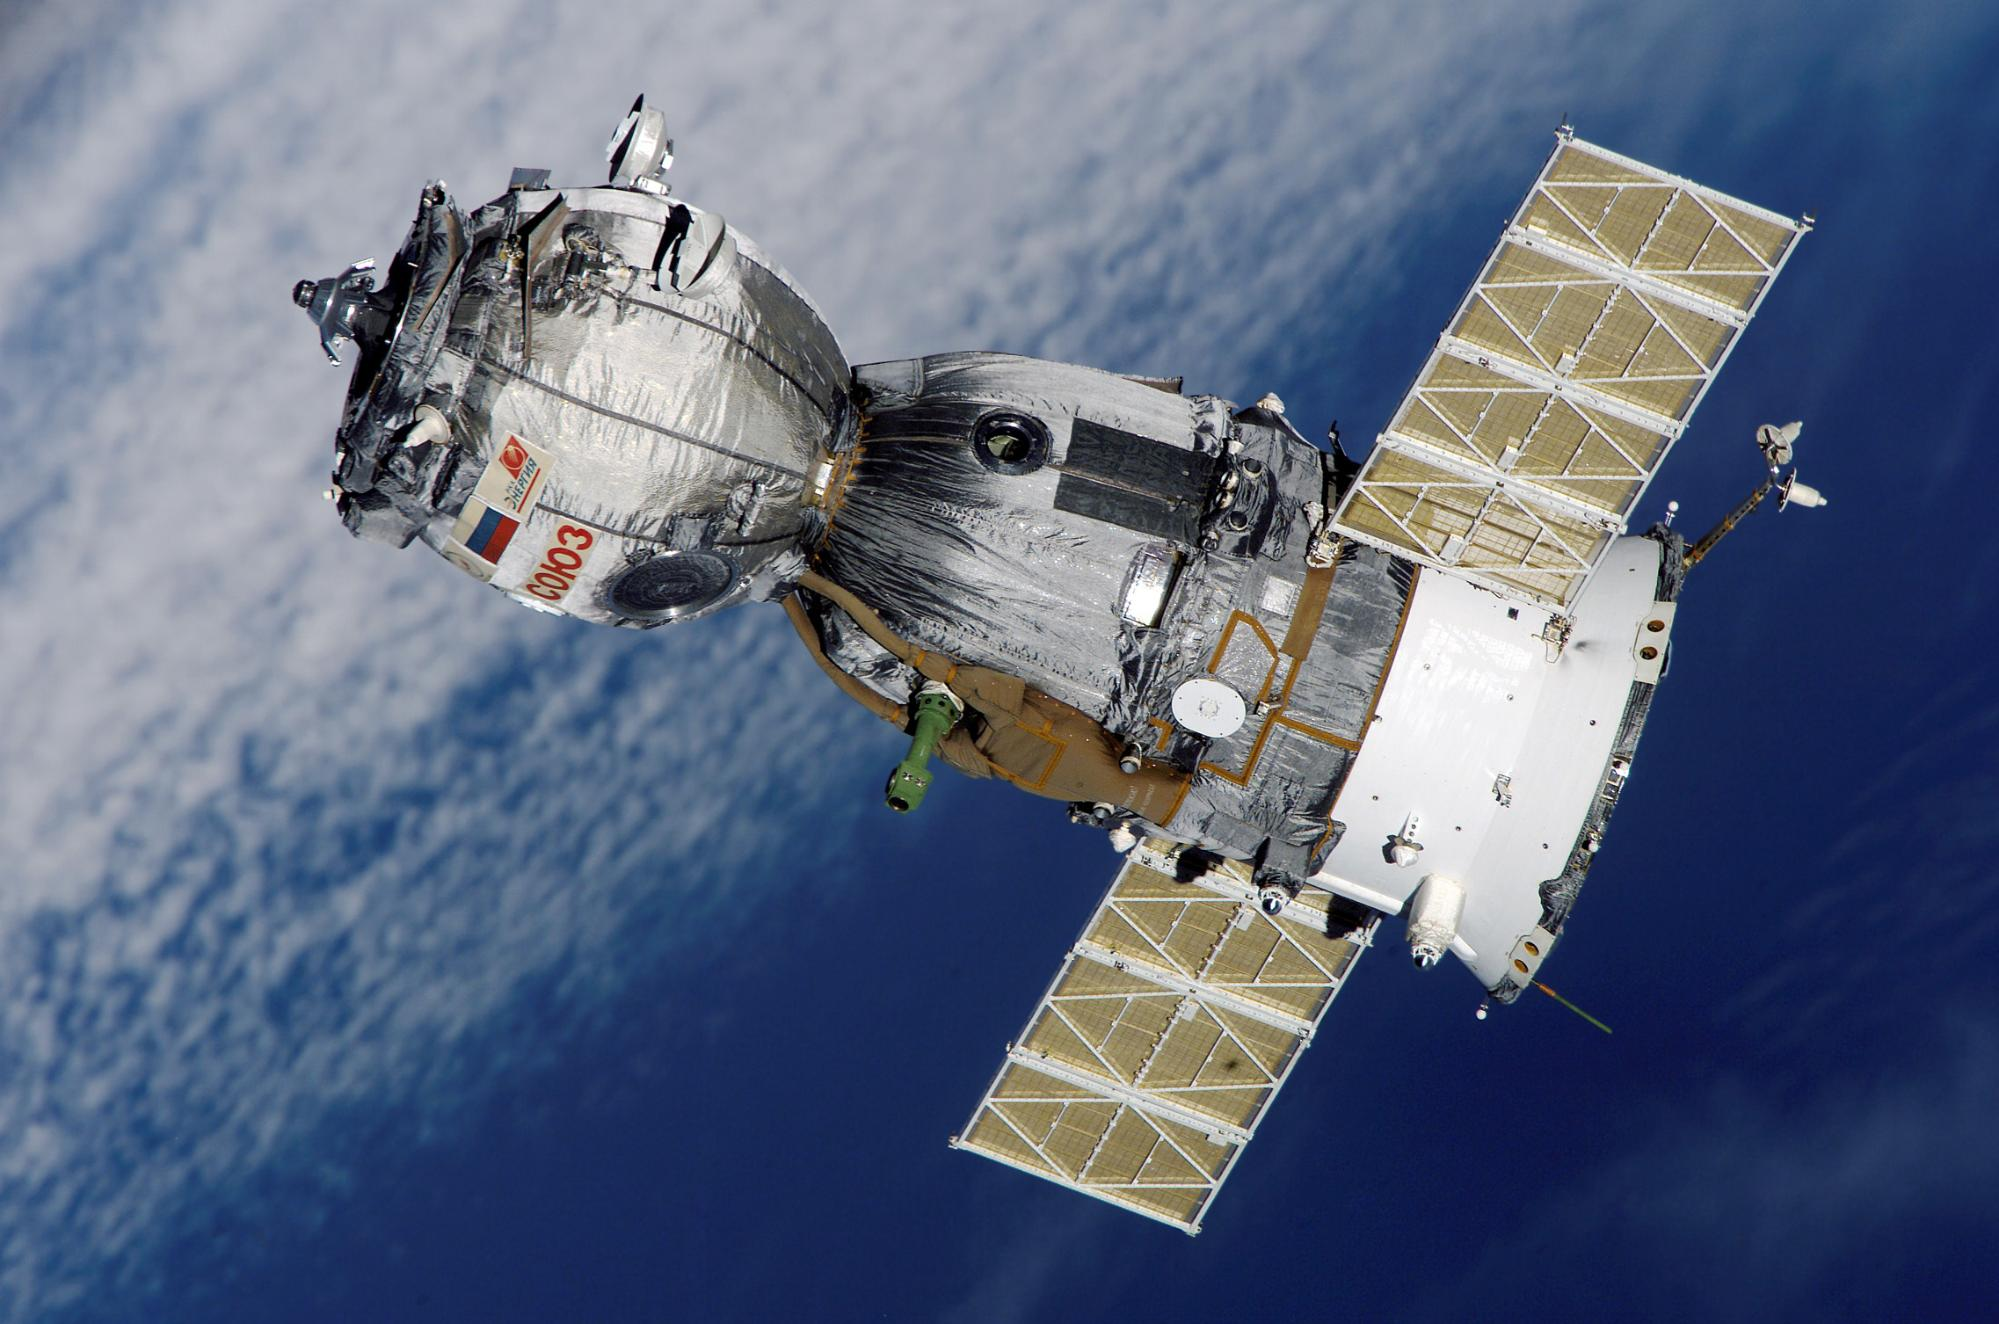
\includegraphics[scale = 0.1]{assets/soyuz.jpg}
 \end{center}
 \end{itembox}
  \subsection{素材について}
 基本的にデザイン局の方と連携を取りながら行っていく。\par
今回の場合はこちらが最初にデザイン案を作りそれをデザイン局の飼沼とブラッシュアップした。\par
 \subsection{各画面について}
 全体として今回矢向は李のアドバイスを勘違いしMainActivity以外全部Fragmentというあまり類を見ない設計にしてしまったので参考になならない箇所もあると思われる。
 \subsubsection{ツールバー}
 \begin{minipage}[b]{13.5cm}
 Androidの機能も用いて作ることもできる。\par
 だがしかしこれだと取り回しがあまりにも悪いので、右図のようにactivity\_main.xmlにて画面をLinearLayoutで分割し、上(赤い部分)にはツールバー、下(青い部分)をRelativeLayoutにしてFragmentContainerにし、ここだけでフラグメントを置き換えるようにするとフレキシブルなツールバーを作成できる。詳細は以下のリンクから。\par
  \url{https://qiita.com/mi_iroha/items/c8b6a1a6262c77e28301}\par
  この時普通のツールバーのメニューはどのように出すのかという疑問が出るかもしれない。結論としてはDialogFragmentを継承したダイアログを位置を右上などに指定して出す(指定方法は調べればすぐに分かるので割愛)。
 \end{minipage}
 \begin{minipage}[t]{3cm}
 
\includegraphics[width=3cm]{assets/ToolBar.png}
 \end{minipage}\par\par
ツールバーのonClickの実装を各Fragmentでしなおすことで(今回は各FragmentのinitToolBar()やonCreateViewにてその処理を行っている)各画面で違ったクリック処理を行うことができ、またその際に現在のFragmentのメンバ変数などにアクセスすることもできるようになる(匿名クラスを使えばより楽にonCreateView()内の変数にアクセスできる)。
今回はActivityがひとつなのでこれだけで無事に作成することができたがActivityが複数ある場合はもう少し工夫が必要だと思われる。
 \subsubsection{ホーム画面}
 ImageViewおいてclickのListenerつけるのみ。難易度はかなり低い。
 \subsubsection{展示一覧}
 RecyclerViewを配置するだけではあるが、絞り込み機能があるため少し難易度が高い。\par
 全展示団体のデータをDB(と今回は混雑度のサーバー)から取得し表示する。\par
 その際にRecyclerViewのAdapterに渡すListを作るとき、絞り込み条件に合致しないものはforループの最初にcontinue文で弾けばよい。
 \subsubsection{食品一覧}
 RecyclerViewを配置するだけ。メモ帳が理解できていればかなり難易度は低い。

 \subsubsection{マップ}
 まず地図の画像はパンフが出来上がったらその画像を使うとよい。出来上がるまでは途中経過の地図を使ってプログラムを書いてく。地図の画像、展示団体等の位置を識別するための画像、ピンの画像、タブレイアウトをおくためのFragment、タブレイアウト内に表示するためのFragment、タブレイアウトの機能を実装するためのAdapterはおそらく必要となる。加えて、地図の操作を行うためのカスタムビュー等も用意することになるだろう。\par
 次に、各機能の詳細について書いていく。\par
 タブで階数ごとに違うマップを出すようにする。タブレイアウトはここをみればわかると思うので詳細は省略する。\par
マップのドラッグ、ズームについては画像をMatrixを使用して移動、拡大縮小するのがよい(画像の座標や、拡大率とかを保存しておくと後々楽になり、Matrixならそれらを保存してくれるから)。描画方法はimageViewを用いる方法とcanvasを使用する新しくViewを作って用いる方法などがあるが今年はimageViewを使用した。どちらもMatrixを使用して移動等が可能。ドラッグやズーム等の検知はGestureDetectorを使って検出した。ドラッグはonScroll、ズームはonScaleで係数を取得することが可能。地図の端に到達した判定は、どこを端と定義するかによるが、今年は「画像の端がスクリーンの真ん中を超える」という判定とした。地図の端をどう定義するかは、色々な外部のサービスを参考にすると良い。慣性は余裕があるならば実装するのが良いが、少し厄介であるため無理して実装しなくてもよい。今年は慣性をonFlingで取得しTimerで動かした。また、画像の端を超えたあとや、ズームで縮小しすぎたあとに戻す処理でもTimerを使用し、滑らかな動きを実装した。\par
マップの操作云々を調べて自分なりの実装が難しいと感じたら李のQiita\footnote{\url{https://qiita.com/Cyber_Hacnosuke/items/b2a8724218d2f4a4c3c2}}を参考にしてください。\par
「タップした場所がどこなのか」を判別する方法は、別途、各展示、食品で色分けされた画像を元に判別する。タップしたスクリーンの座標から、画像の位置座標と拡大率を用いてタップした画像の中の座標を算出し、色分けされた画像のその座標が何色かで判別する。今年は、\verb+ #FF00XX(XX / 2 = id) +が展示、\verb+ #00FFXX(XX / 5 = id) +が食品と決め、色識別用画像を作成した。画像を作るのは自分でやったが、信頼できるなら後輩に頼むと仕事が減る。色識別用画像を作る際、拡大縮小等でボケて、想定していなかった色が検出されないよう気をつけること。\par
詳細画面のピンの座標はデータベースに0~1の範囲で、x,y座標それぞれの割合を記録しておき、表示する際その値から画像用の座標を計算しピンを指してる。この0~1の範囲の座標を計算するにあたり、スプレッドシートを使って計算するのがもっとも効率的と思われる。参考程度に今年使った自分用スプシを\footnote{\url{https://docs.google.com/spreadsheets/d/17zJ-jk277xVDzQYN9v_pF8ZatII3OxnX1dlLHyxBX6o/edit#gid=808228009}}置いておく。\par
最後に、地図を表示するには、大きな地図の画像を用意する必要があるが、その際に重すぎて落ちないよう気をつけること。\par
 \subsubsection{タイムテーブル}
 1イベントあたりのレイアウトを別途xmlで記述しておく。\par
また、今回の場合は9:00の線と10:00のy座標から1時間あたりの座標変化数を取得しておく
DBから表示すべき全イベントを取得し、それぞれのイベントごとにfor文を用いて先程のxmlファイルをLayoutInflatorでインフレートし、各イベントの開始/終了時間と先程の値を用いてそのViewのTop,Bottom,heightを計算し表示(ViewGroup.addView(View)みたいなのでできる)するとよい。\par
Viewの生成はここを参照することを推奨する。
 \subsubsection{トレジャーハント}
 ここに関してはおそらく設計者が次回も(そもそも次回もトレハンをやるのかという問題があるが)ITECの人間ではないので少々我々プログラマサイドからではわかりにくいかもしれない。\par
 いかに内容を噛み砕いて実装できるかが成功のカギとなる。\par
 実装自体の難易度はあまり高くない。
 \subsubsection{聖光ラジオ}
 HTTP通信で取得した内容をRecyclerViewで表示するのみ。\par
 応募に関しても、応募する内容をHTTP通信で送るのみのシンプルな処理。
\subsection{各技術指導}
 \subsubsection{HTTP通信}
 難易度はかなり高い。\par
 この引継書もこれを書くために書いたと言っても過言ではない。\par
 OkHttp3という外部ライブラリを使用した。\par
 implementation group: 'com.squareup.okhttp3', name: 'okhttp', version: '3.14.9'\par
 Gradle(build.gradle(app))に上記の内容を書いておく。\par
 プライバシーポリシーにもokHttp3使用の旨を書かなくてはいけない。\par
 Android(というかGoogle)は画面の描画が遅れフリーズなどをしているようにユーザーに感じられてしまうのを防ぐため、通信処理をメインスレッドで行うとNetworkOnMainThreadExceptionという例外を投げるようになっている。\par
 つまり通信処理はマルチスレッドで行わざるを得ない(こう書いてはいるが通信は別スレッドで行うのがセオリーなのでこれはおかしいことではない)。\par
 JavaやKotlinでマルチスレッド処理を行うには、Threadクラス等を継承もしくはRunableインターフェースを実装したclassのrun()メソッドをオーバーライドし、その中にマルチスレッドで行いたい処理(今回なら通信処理)を書くことになる。\par
 とはいっても今回出してもらったプログラムを見る限り半年でこれを自力で行えるレベルに到達するのは(勉強などを考えると)かなり厳しいと思われるのでFragmentと連携して通信内容を表示する雛形を載せておく\footnote{\url{https://qiita.com/Jellyfish4594/private/9709ad41d0828f917601}}。
 \subsubsection{RecyclerView}
 \begin{enumerate}
 \item list\_item.xml
 \item RecyclerViewHolder
 \item (保持する値が複雑な場合は)RecyclerStructure
 \item RecyclerAdapter
 \item 表示する
 \end{enumerate}
 の順に作れば5~10分で作り終えることができる。\par
 ここ\footnote{\url{https://qiita.com/Todate/items/297bc3e4d0f3d2477ed3}}の内容をほぼコピペで使用することができるが、Adapterのoverrideメソッドの引数に一部が本来はあっていはいけない?がついているため、そこだけエラーが出る(もとのメソッドの引数がnull許容型ではないからエラーとなる)。
 \subsubsection{QRコード}
 そこそこに難易度が高い。\par
 これ\footnote{\url{https://github.com/SeikoStudentCouncil/SeikoFestaAndroidApp62nd/blob/master/app/src/main/java/jp/ac/seiko/itec/seikofestaapp62nd/fragments/treasurehunt/QRCodeFragment.kt}}をコピペするだけで大部分を完成させることができるが、下記のようにGradleに書かなければならないので注意(ZXingを入れる、OkHttp3と同様にプライバシーポリシーにも書く)。\par
 implementation 'com.journeyapps:zxing-android-embedded:3.6.0'
 \subsubsection{Fragmentを一部に表示}
 RelativeLayoutを配置しそれをFragmentContainerにすることでできる。
 \subsubsection{GoogleMapを置く}
 ここ\footnote{\url{https://developers.google.com/maps/documentation/android-sdk/start?hl=ja}}に従う。
\subsection{リリースについて}
\begin{itembox}[l]{Google開発者用アカウント}
\color{red}
mail: seikosougiken@gmail.com\par
pass: gikenmember
\end{itembox}
これがないとリリースができず詰みとなってしまうので気をつける。
\subsubsection{審査について}
李のとき(第60回)は2\UTF{FF5E}3時間で終わったと聞いて油断していたが今回は現在審査に出して72時間ほど経つがいまだ終わっていない。2019年の9月あたりから審査が厳正化しているそうなので気をつけるように。今回もそうだが素材がなかなか来ないのでASAPを心がけるだけでよい。ちなみに審査はおそらくカルフォルニアで行われている。
\subsubsection{審査時間の目安}
初回審査...72時間程度=3営業日(遅い場合は問い合わせも手)
それ以降のアプデ...1営業日(カリフォルニアの)
\subsection{後輩の育成について}
正直なところ、聞かれたらいくらでも教えてあげることはできるが\textbf{\gtfamily 体系的に教えてあげることができるのはせいぜい} 基本制御構文\footnote{if文やfor文などのこと}や変数などの
\textbf{\gtfamily 全プログラミング言語に普遍的に存在する概念くらい}で、オブジェクト指向やアプリの本格的な作り方などの習得度合いは\textbf{\gtfamily 学ぶ本人の主体性}に依るところが多いと思われる\footnote{おそらくプログラミング系統だけではなくて動画やモデリングなどでもそう}。
ここだけの話「もう来年以降の技術は知らん()」といった会話もよくあった。この手の技術の習得には自分で練習することが必要不可欠だし、ここあたりは勉強に通ずるところもある。よって教える側ができることは
 \begin{itemize}
 \item 質問には必ず答えてあげること
 \item 自分が学ぶときにしてほしかったことをしてあげること
 \end{itemize}
の2点だと思う。
逆に真面目にやりさえすればプログラミングスキルなんて\par
文法+ライブラリの使用方法の知識\par
にほかならないので習得は(オブジェクト指向などの一部の関門を除き)習得は容易だと思う。\par
技術的な習得レベルの目安としては、最低限メモアプリを自力で作ることができなければアプリを「ちゃんと」任せるのは厳しいかもしれない、といった感じ。
 \subsection{おまけ1:小技(よくあるちょっとしたエラー)}
 \subsubsection{NullPointerException :\UTF{FF5E}Attempt to\UTF{FF5E}という例外が発生する}
 多くの場合findViewByIDをする際の引数のidが間違っている(findViewByIdしているviewの中に存在しないviewを探そうとしているためnullが返されてしまう)。\par
xmlやktをコピペした際にidを変え忘れたり、xmlの場合はDesignタブでコピペしたidを意図したものに直そうとするとAndroidStudioがリファクタリングと勘違いしコピペ元とコピペ先両方のファイルのidを変えたりすることで起こる。findViewByIdは該当するviewが見つからないとnullを返す(らしい)ので代入先がnullableでなかったりする場合に起こる。
 \subsubsection{宣言部参照}
 メソッド名や変数名をctrlを押しながらクリックすることでその宣言部にジャンプすることができる。\par
自分が書いたコードでなくても(例えばandroid.view.Viewクラスなどでも)可能。
・使用箇所確認
メソッドやクラス、変数の宣言部にてその名前をctrlを押しながらクリックするとそれが今開いているプロジェクトのどのファイルの何行目でどのような引数で使用しているかを一覧として表示することができる。

\subsubsection{Database Inspector}
アプリ実行中(DBを使用すれば)下のバーの「App Inspection」からDBの中身をExcel形式で見たり編集したりできる。また任意のSQL文を実行することもできる。デバッグに便利。\par
実行している端末のAPIレベルが低すぎると使えない(確か26以上)。
\subsubsection{Layout Manager}
右下の縦のバーにある。アプリ実行中に使うと現在開いている画面がどのViewで構成されているかが分かる。面白いけれど個人的には役に立ったことがない。実行している端末のAPIレベルが低すぎると使えない(確か26以上)。
\subsubsection{Profiler}
下のバーにある。実行中に現在どれぐらいメモリやCPUのリソースを消費しているかが分かる。
\subsubsection{OutOfMemory}
DBの場合ちゃんとcursor.moveToNext()しているかを確認する。\par
画像を扱っている場合dpi別に画像をリサイズしてdrawable-hdpiやdrawable-mdpiなどに分けて入れておくとAndroid側の処理の負担が大幅に軽減できる。リサイズ作業はpythonを使えると楽に済ますことができる。
\subsubsection{context}
多くの場合困ったときにはこれに必要なものが入っている。\par
このクラス正体は、現在表示しているActivityの情報(ツールバーは表示する?画面のテーマは?など)が入っているもの。Fragmentからアクセスしたい場合はrequireContext()でできる(同様にrequireActivity()とかある)が、メソッドの中で使用しないとエラーが出る(onCreate()あたりが呼ばれないとcontextはまだnullであるから。どうしても使いたい場合はcontextを引数で渡す)。
\subsubsection{PreferenceEditor}
DBに入れるほどでもないがアプリが終了しても保存しておきたいデータを入れられる。
しかしかなりの頻度で読み出しに失敗してしまい、我慢ができなくなった矢向はほぼ同じ機能をもったclassをjsonベースで作成しそれを使用した(ファイル読み書きはほぼ確実に行われる)。
\subsubsection{使えると便利な言語}
GAS(JavaScript)とpythonは書けることが望ましい。(英語は言うまでもなく読めたほうがよい)。
\subsubsection{ConstraintLayout}
なぜかL4で使う人が多く見受けられた。
基本的にはFrameLayoutとLinearLayoutで全て済ませられると思われる。
個人的にConstraintLayout使うのは初心者とすごい手練だけな気がするので、自分がよほどの上級者である自信がないのなら使用には気をつけることを推奨する。
\subsubsection{信用できるサイト(よく見るサイト)}
エラーで停滞しているときは矢向自身個人ブログなどもよく参照しているしよいと思うが、エラーというわけではないちょっとした調べ物のときに優先的に参考にするサイト
\begin{enumerate}
 \item Qiita
 \item 侍エンジニア
 \item teratail
 \item techacademy
 \item stack overflow
 \item Google公式
 \end{enumerate}
\subsubsection{うまく実装できないとき}
なるべく細かい機能に分割して1つ1つ別のプロジェクトで作り最後に統合する。例えばメモ帳ならDBだけ練習、RecyclerViewだけ練習、fragmentの遷移だけ練習、とするとよい。
\subsubsection{エラーが治らないとき}
Logをたくさん出すor上述のように別のプロジェクトで試してみる。
\subsubsection{Fragmentが透けたり、Addしてるときに下のFragmentも反応しやがるとき}
前者の場合はレイアウトファイルの一番上のFrameLayoutとかのbackgroundをcolorのwhiteにしてしまえばよい。\\
後者の場合はその反応してしまうfragmentのレイアウトの一番上のFrameLayoutを事前にfindViewByIdしておき、addする瞬間にvisibilityをINVISIBLEに設定し、画面が復帰したときにVISIBLEにすればよい。ViewがINVISIBLEになるとユーザーからの操作を一切受け付けなくなる性質を利用する。publicメソッドにしておいて、FragmentTransaction.fragmentsからインスタンスを取得してそのメソッドを呼び出すことでできる。
\subsubsection{DBについて}
DatabaseOpenHelperは1つまでしか作れない(おそらく)。
個人的にこの名前は良くないと思う。
Helperとは書くけれどこれを使う以外の方法でDBにアクセスする現実的な方法はないと思われる。補助的な印象を受けるがしっかり主軸として運用することになる。
\subsubsection{ImageViewにdrawableの画像を名前で指定して表示する}
知らないと停滞することになる。矢向の記事\footnote{\url{https://qiita.com/Jellyfish4594/items/2ddf3d6f1bcef66fedf2}}(ほぼ李のノウハウ、最も李でなくても広く一般的に使われている方法だが意外と調べても出てこない)を参照のこと。
\subsection{おまけ2:矢向のブラウザのブックマークのAndroidフォルダにあるリンク}
コピペしていくらでも使い回せるものなどが多いので見ておいて損はないかもしれない。
(一部ただのGoogleドライブのリンクとかは消してある)
\begin{itemize}
\item お問い合わせ - Play Console ヘルプ\\
\url{https://support.google.com/googleplay/android-developer/gethelp?hl=ja&visit_id=637678981545128687-2809304254&rd=1#}
\item Android開発で困った時の問い合わせ先 | アプリ開発のお勉強! アプリリ\\
\url{https://bit.ly/3on3bmL}
\item Shrinking your app with R8 (Android Dev Summit '19) - YouTube\footnote{\url{}{}}\\
\url{https://www.youtube.com/watch?v=uQ_yK8kRCaA}
\item Androidアプリの初回リリースを手動で公開する方法に関するメモ - AppSeedのアプリ開発ブログ\\
\url{https://develop.hateblo.jp/entry/google-play-manual-release}
\item Y.A.M の 雑記帳: 3月 2014\\
\url{http://y-anz-m.blogspot.com/2014/03/}
\item 大容量のビットマップを効率的に読み込む  |  Android デベロッパー  |  Android Developers\\
\url{https://developer.android.com/topic/performance/graphics/load-bitmap?hl=ja}
\item コピペしてすぐ使えるアラートダイアログ集 - Qiita\\
\url{https://qiita.com/suzukihr/items/8973527ebb8bb35f6bb8}
\item 【Android】 AppCompatActivity の ActionBar のタイトルを動的に変える: スタジオプリズム\UTF{3427}3ブログ\\
\url{http://s-prism3.seesaa.net/article/438905821.html}
\item 【Android】カスタムダイアログを作った。: Java知識ゼロ人間の生活\\
\url{http://stren-blog.seesaa.net/article/367038846.html}
\item アプリバーを使用する  |  Android デベロッパー  |  Android Developers\\
\url{https://developer.android.com/guide/fragments/appbar?hl=ja}
\item AndroidXに対応しようとしてハマった話 | 株式会社ブリッツゲート\\
\url{https://blitzgate.co.jp/blog/2350/}
\item 【Android】XMLファイルからViewを生成する - プログラマーのメモ書き\\
\url{https://bit.ly/3wDqZq9}
\item AndroidでSqliteデータベースを操作する - Kotlin編 - Qiita\\
\url{https://qiita.com/NaoSekig/items/0d95d631378040c1961a}
\item Android:TextView・Button等に角丸や枠をつける - asky\\
\url{https://asky.hatenablog.com/entry/2016/05/04/194303}
\item 【Android】selecterを使ってみる - It’s now or never\\
\url{https://inon29.hateblo.jp/entry/2014/01/13/184153}
\item GASをWeb公開して実行(doPostとdoGet) | アンクルエンジニアの気づき\\
\url{https://uncle-atsushi.com/gas_first-execute_dopost-doget/}
\item Android アプリ公開時に必要な画像リソースをサックっと用意する手順まとめ|itog|note\\
\url{https://note.com/itog/n/n5253e8d28d2d}
\item Android用画像読み込みライブラリ、Glideを使ってみよう! | 株式会社ヌーラボ(Nulab inc.)\\
\url{https://nulab.com/ja/blog/nulab/android-library-glide/}
\item 【Kotlin】 Zxing QRコードリーダーをカスタマイズ - Qiita\\
\url{https://qiita.com/Mosea/items/e9dae626713fe9950734}
\item 【コピペで作る】kotlin QRコード導入手順5ステップ\\
\url{https://shoheohtani.blogspot.com/2019/01/kotlin-qrcode-how-to.html}
\item テキストから読み取った画像ファイル名を表示したいです。 - Yahoo!知恵袋\\
\url{https://detail.chiebukuro.yahoo.co.jp/qa/question_detail/q11153402421}
\item KotlinでAndroidのカメラ機能を利用する - Qiita\\
\url{https://qiita.com/naoi/items/04e44308221f6eb73024}
\item KotlinでGoogle Sheets API v4を使う | キャスレーコンサルティング株式会社\\
\url{https://www.casleyconsulting.co.jp/blog/engineer/4798/}
\item ビルド環境の設定
\item 【Android】Fragmentを使うときのコツとか色々 - Qiita\\
\url{https://docs.kii.com/ja/samples/push-notifications/push-notifications-android-fcm/configure-ide/}
\item 【Kotlin】Bundleを使ったFragment間の値渡し - Qiita\\
\url{https://qiita.com/HideMatsu/items/ddf640899cbe1b2027ed}
\item Android はじめてのFragment - Qiita\\
\url{https://qiita.com/orimomo/items/0472a52f90d14bef0c89}
\item 文字列リソース  |  Android デベロッパー  |  Android Developers\\
\url{https://developer.android.com/guide/topics/resources/string-resource?hl=ja}
\item KotlinでRecyclerViewを使ったリスト表示を行う - Qiita\\
\url{https://qiita.com/Todate/items/297bc3e4d0f3d2477ed3}
\item KotlinでのFragment実装方法 生成と切り替え | Memento Mori Blog\\
\url{https://memento-mori-blog.com/android-kotlin-fragment/}
\end{itemize}


\newpage
\section{音楽局}
\subsection{引き継ぎにあたって}
引き継ぎは、来年もやりたいようにやってほしいと思っているのであまり書くことはないのですが、技術部門で音楽を担当していた人としての認識、知ってほしい知識について少し書こうと思います。

さて、「音楽」の名前を冠する部署として、まず音楽とは何かを見つめ直す必要が出てきます。
現状、局長個人の見解としては、最も簡単かつ漏れのないようにその定義を行うならば、音楽とは「作曲」「上演」「享受」の3つに分類されて考えられるべきもので、したがって技術部門の音楽担当としても、その区分を意識した上で自らが行うことを決めていくべきだと考えています。それぞれについて知っておくべきことを書きます。

\subsection{作曲}
「作曲」の作業は、言うまでもなく曲を作ることで、音組織を自分で設計して、一つの曲となるようにしていくことで、当然音楽を担当する身として最重要のことがらであると考えて良いです。この技術は専門性、独創性の両方が求められる難しい作業なので、 参考書籍をいくつか羅列するにとどめます。この作業はパソコン上でも、紙の上でも、頭の中でも行えるため、実務上引き継ぐことは特にありません。
ただし、2つだけ確認したいことを書きます。
まず、動画との連携についてはいくつかスタイルがあるということです。第62回聖光祭スローガン発表動画では、絵コンテを待って音楽を作り始めて、動画と音楽が揃うようにお互い合わせながら制作しました。1番楽なスタイルは先に音楽を提出してそれに合わせて動画がすべて作るという形ですが、これは個人の好みや動画のコンセプトによって変えるべきだと思うので、探求してください。
次に、音楽は強く全体の空気感をコントロールするということです。スローガン動画やオープニング動画では前進を意識して音楽緊張状態を多用したり、エンディングでは安定した和音を使ったりするなど、音楽的工夫が自由にできるようになると、音楽自作の意味がやっと出てきます。\\

{\bf 参考書籍}
\begin{itemize}
  \item 石桁真礼生 他『楽典 理論と実習』(1998)\\音大受験をするのでなければ内容を網羅する必要は全くないですが、そもそも音楽を学ぶにあたって必要な用語や論理が理論的に説明されている(ex.完全◯度と長◯度は何が違うのか?)ため、一読して損はないです。
  \item アルノルト・シェーンベルク『作曲の基礎技法』(1998)\\前提知識がある程度要求されるが、「作曲」という作業の骨組みをとるにあたって本当によくできた名著。前半だけでも読む価値あり。高い本なので言ってくれたら貸します。
  \item 清水響『コード理論大全』(2018)\\ナナメ読みしたことしかないですが、おそらくバークリーメソッドを基本にコード理論がよくまとまっている印象を受けました。ただこの分厚さなので、辞書くらいの気持ちで使うのが賢明だと思います。
  \item これら参考書籍にどっぷり浸かる前に、soundquest\footnote{\url{https://soundquest.jp/category-archive-chord/}}
  という音楽理論の講義に無料アクセスできるサイトがあるので、これを片っ端から読むのが案外近道だと思います。
  名曲を期待しています。
\end{itemize}

\subsection{上演}
「上演」というのは、ここでは「音楽が(生)演奏・再生されること」として考えます。ここでは今年うまく回りきらなかった、引継ぎたいことがいくつかあるのでしっかり読んでほしいです。
まずは「演奏」についてです。聖光祭(あるいは他の学校行事)で音楽が演奏されるとき、合奏形態をとるならば、多くの場合編曲作業が必要です。既存曲の流用にしても、生演奏を標榜するならば、集められるメンバーによって演奏できるような形式(合奏なら編曲した上でパート譜が必要、など)に音楽を編集して、奏者に渡すことが必要です。
62回聖光祭では、生演奏による演出が複数行われましたが、たとえばグランドフィナーレ第2部オープニングでは混乱の中でパイレーツオブカリビアンを生演奏することが決まって、演出部門長が自力でパート譜を作成して配るなど、そのプロセスは技術側ではほとんどコントロールできていなかったのが実情です。企画、演出の各部門と連絡を取り合って、誰に何ができるのかを常に共有し合う必要があります。技術としてグランドフィナーレには最初から積極的に絡んで、演出、放送の各部門と連携して企画部門の動向を把握しておくつもりで参加した方が良いものになると思います。
次に「再生」に関してですが、ここでは「作曲」から独立した、音響調整の作業を行う必要があります。これは制作サイドの話で、パソコン上で行う作業がほとんどなので技術的な問題しか存在しないのですが、音響調整に含まれるミックスダウンとマスタリングは局長自身も素人なのであまり具体的なアドバイスはできません。正直プロにはどう頑張っても設備の問題で勝てないので、予算でマスタリングスタジオを借りるというのもありなくらいだと思います。ただ、再生される場所が講堂なのか、外ステなのかなど、校内の環境によって音響調整を変える、などの作業は自分達で行うしかないので、ある程度音響についての知識は持っておくべきだと思います。なお、生演奏の音響については、聖光祭では演出部門でPAさんを呼んで行っているので特に気にする必要はありません。

\subsection{享受}
「享受」が音楽の一部として認められるのかという疑問は、藝術学の話題に踏み込んでしまうので放置しますが、ここでは音楽がエンターテイメントとして成立するための、音楽以外の事柄について少しだけ書きたいと思います。
重要なのは、誰がどんな場所で音楽を享受するのか、ということです。第62回聖光祭のグランドフィナーレオープニングでは、生演奏を担当しました。あの会場で考えるべきなのは、観客の皆さんの拍手がどう音楽に混ざるのか、など、享受者と音楽の関係についてです。聖光祭では、音楽が享受されることを常に意識しながら作業してください。それは照明演出との連携など、多くの要素を含みます。先述の通り馬の空気感をコントロールするのは音楽です。総合演出にまざるときには積極的に参加することをお勧めします。

\subsection{-}
今回は初年度ということもあり仕事がうまく振れないなど迷惑をかけましたが、来年からこの部署が聖光祭で大きく活躍してくれることを願っています。以下は、細々とした事項を羅列しますが、来年は来年として、また新しい形の聖光祭における音楽の役割が生まれることを期待しています。

 \section{アプリ局(iOS)}
 2019年以前はiOS開発者がAndroid開発者より圧倒的に多かったが、2021年はiOS開発者が圧倒的に少なく、三枝と李のたった二人でやっていた。
  \subsection{言語}
  第62回聖光祭ではiOSアプリ制作にSwift、またUIの作成にはSwiftUIを使用した。第60回以前の聖光祭アプリではSiwftとStoryboardという一般的なアプリの構成だったが、Sotryboardの扱いが大変なのに加え、アニメーションを強化したかったので、2019年に新しく登場したSwiftUIを使用した。
  \subsubsection{Swiftの学び方}
  \url{https://apple.co/3BVig3C}
  \url{https://developer.apple.com/tutorials/swiftui}
  \url{}
  \subsubsection{SwiftUIの利点}
  \subsubsection{SwiftUIの問題点}
   たまにプレビューが機能しなかったり、重くてXcodeが間違ったコードをハイライトしてくれないと言った不具合があった。あとはSwiftUI自体がコードが複雑になって重くなると、正しいコードを書いているのにプレビューされなかったり、ビルドに失敗したりした。大抵の場合は``Clean build Folder''かXcode再起動で解決する。\\


 \section{デザイン局}
 \section{特別業務}
 \subsection{名簿}\label{sec:名簿}
62回担当者:飼沼、浅井、李、古澤 他\vspace{3mm}

4月になったら技術局管轄の全校名簿を作ろう。飯岡先生に名簿をいただけないか交渉して、無理だったら全員分の情報を職員室の短冊を見ながら手打ちで差し替えよう。学籍、氏名(異体字に注意!正確に打ち込むこと。姓名間は半角スペースで管理)、学年([J,S][1-3])、クラス、番号、メールアドレスを対応させる。執行部、部門長、生徒会役員等々は見れるようにしておいてもいいが、セキュリティに厳重注意!!流出した瞬間クビだと思え。

部門動向本調査では、回答結果を上手く編集して所属一覧を作成した。この部分は統一シフト({\bf\ref{sec:統一シフト}}参照)に深く関わったので、李が主に行った。食品は店舗(店舗の識別番号および略称を作るとよい)、企画は各企画、展示団体員は展示団体(展示団体の識別番号および略称を作るとよい)まで最終的に記録する。なお、幹部のは執行部が掛け持ちを精査し、許可するので、掛け持ち希望シートを作成して幹部全員にそこに記入させよう。演出だけ注意({\bf\ref{sec:演出部門}})。
執行部管轄、各部門管轄、先生管轄の所属(ex. 弦オケ、吹奏楽部、合同演奏、Mサロ、選択芸術展示、企画出演、グラフィナ、などなど...)は整理して事前にまとめておこう。これらにも識別番号と略称を付与しよう。




 \subsection{議事録班}\label{sec:議事録班}
62回担当者:飼沼、浅井、李 他

 \subsection{YouTube関連}
62回担当者:三枝、向山 他
\\
\\
 部門長(副部門長)や展示団体のインタビューや、活動風景などを投稿する。
 第61回からこの企画は始まったが、YouTubeへの投稿が聖光祭1~2ヶ月後になってしまうなどといった問題がある。YouTube企画専門のチームを作るといいと思った。
 第62回聖光祭副実行委員長のコメントを載せる。
 \\
 \\
 \begin{itembox}[l]{第62回聖光祭副実行委員長 向山 雄登より}
 引き継ぐことは何もありません。\\
 ただYoutubeはやった方が良いと思います。\\
 61期の中で管理者の代表を決めたら僕に教えてください。チャンネルの権限を付与します。ちなみになぜか聖光メールアドレスでは出来ないっていう設定になってます。あとはその代表者が勝手に他の人なりを自由に追加してってください。\\\\
当日まで、いろいろ撮ってみると良いと思います。インタビューもあり、展示団体等の準備に密着してみるとかは面白いと思います。撮影経験を積んでおくという意味でも役に立ちます。\\
問題は当日の撮影です。\\
62回の問題点として、撮影者が少ない。いるが各々別の仕事が入っていてシフトを入れる余裕がない、ということがありました。というかそれがほぼ全てでした。\\
61回はそれでいけてたんですが、それは幹部の仕事が少なかったから可能なことだったんですよね。\\
確実に撮影しようと思ったら絶対に撮影専門部隊を作ることをオススメします。\\\\
校内を回って写真撮っていく部隊ではなく、講堂・小講堂・外ステなどある程度決まった場所でカメラを管理します。んじゃあ楽じゃんと思うかもしれませんが、バッテリーをどのタイミングで交換するのかを考えないと当然死にます。\\
講堂は一回席後方にコンセントがあるのでそこから繋げます。外ステはベランダから撮るなら外ステの対角の2回ベランダにコンセントがありますが、ベランダから撮るより前で撮る方が絶対に良いと思います。\\\\
正直あんま需要ないんじゃね?と思ってもいましたが、YOUTUBEに挙げる挙げない関わらず良い機材で撮影してあげるというのは需要があります。なので頑張ってください。
 \end{itembox}


 \subsection{情報公開}
62回担当者:飼沼、浅井、李、劉、古澤、永井 他



 \subsection{ストリートピアノ}
62回担当者:満田 他

 \subsection{コロナ対策}
62回担当者:飼沼、深代 他

 \subsection{グラフィナ}
62回担当者:満田、三枝、飼沼 他

 \subsection{震災対策}

 \subsection{舞台演出}
62回担当者:満田、三枝、飼沼

 \subsection{アイデアソン}

 \subsection{サインデザイン}
62回担当者:飼沼

 \subsection{ワークスペース講座}
62回担当者:飼沼、浅井、李

 \subsection{英語表記統一}

 \subsection{雨天マニュアル}

 \subsection{生徒総会}
 オンラインで開催される場合は、動画局が動画を作る。\\
 聖光祭に関する連絡や幹部紹介、生徒会役員紹介を流すものが四月、体育祭に関する連絡をするものが九月にある。\\


 \subsection{団体管理}
 62回担当者:飼沼、李

 \subsection{Slackアーカイブ}
 62回担当者:飼沼、李

 \subsection{スローガン}

 \subsection{Tシャツ処理}
 62回担当者:飼沼、浅井

 \subsection{統一シフト}\label{sec:統一シフト}
 62回担当者:李
  \subsubsection{導入前のシフト}
  統一シフトによってどんなことができるようになったかについて書く。統一シフト導入前は主に各団体や部門が作ったシフトをメールやLINEで部門員や団体員に送るという形だった。シフトがダブルブッキングした場合はお互いの長で話し合い、解決していたと思われる。第59回聖光祭ではスプレッドシートを使った初めての統一シフトが行われた。これを旧統一シフトと呼ぶことにする。この旧統一シフトは全団体、全部門に優先順位をつけてその順番に各団体からある程度埋まったシフト表を回収してそれを一つのスプレッドシートに入れていくという作業を何回も繰り返すというものだった。当然それぞれで作ったシフト表なので被りがでてくる。被りはまたその優先度が決められており、基本的には団体の優先順位が適応されるが、昼時の食品店舗や、演目への出演はその部分だけ優先される。負けた場合はそこが入らなかったということを記入してまた団体に返す。そして再び集めるというのを短いスパンで何回も繰り返したそうだ。
  \subsubsection{統一シフトの概要}
  第61回聖光祭から僕が作った統一シフトシステムを運用することになった。結局第61回は内部開催になったので運営はできなかった。それでは説明していく。まず、一番簡単な方法として考えられるのはみんなでスプレッドシートを編集するということである。しかし、編集権限を渡してしまえば好きなような改ざんできたり、形式もバラバラになってしまう。そこで、それをオーバーラップする形でシステムを組んだ。スプレッドシートをわかりやすく表示したり、入力方法を選択制にしたり、ログイン制を実装している。
  \subsubsection{仕事内容という概念}
  ネーミングを適当にしたらそれを報告書に書かれてしまい、そのまままかり通ってしまった用語「仕事内容」に関して説明する。仕事内容とは印刷時に印刷される文字のことでどこで何をするかを端的に表したものである。\verb+A-B-C+の形になっており、 部門であればAに部門名(略称)、部門でなければAには\verb+展示団体、食品店舗、その他+が入る。部門でない場合にはBに団体名(略称)が入る。部門であればBとC、そうでなければCには自由な語を入れることができる。これによって完成した仕事内容は一つの業種として各団体にストックされ、団体は必要な仕事内容をすべてあらかじめ申告する。統一シフト入力サイトでストックした仕事内容の束から選んで入力するのだ。団体それぞれ、シフト入力前に必要となるであろう仕事内容を考えるというわけだ。また、それぞれの仕事内容には優先度が決められており、上書きする場合にはもともと入ってる仕事内容より優先度が高い(同値も含む)もののみ認められる。
  \subsubsection{構成}
  \begin{itemize}
  \item Google Spread Sheet\\
  DB。データを格納する。
   \item Google Apps Script\\
   DBからデータを抽出したり参照したりしてログイン、統一シフトの取得と編集、仕事内容の取得などを行なっている。サーバー代わり。
   \item Nuxt.js + Scss + Typescript\\
   Webサイトの構成。Nuxt学んだし、王道な構成でやろうと思った次第。
   \item jQuery\\
   Ajax通信したいので入れた。
   \item Firebase\\
   作ったWebサイトをホストするためにFirebase Hostingを使った。
  \end{itemize}
  \subsubsection{統一シフト関係のスプレッドシート}
  地獄である。
  \begin{itemize}
  \item 統一シフト\\
  統一シフト。1日目、2日目、3日目のシートがある。列はシフト開始時間(10分単位)、行は学籍番号を表している。列の初めのいくつかの列は順番とか決まってるので変えないこと。変えるのならばGAS側とWebサイト側も変える必要が出てくる。
  \item 関連情報一覧\\
  ログイン情報と仕事内容一覧が書いてある。運営中はここを主に編集することになる。書いてあるものが動いているのでここから抜けばログインできなくなったり、仕事内容一覧に表示されなくなったりする。
  \end{itemize}
 \subsection{入場システム}
 \subsection{オンライン食品予約システム}
 \subsection{講堂予約システム}
 \subsection{電子決済}
 今年度導入された電子決済では、Squareという企業の機器を用いている。\\
 クレジットカードから交通系ICまで幅広い決済方法に対応している。\\
 
\includegraphics[scale=0.15]{assets/square_availability.png}
 \subsubsection{注意事項}
 Squareを用いる上で注意事項がある。
 \begin{enumerate}[注意1]
  \item 手数料が発生する\\
  第62回聖光祭では、執行部予算で合計で二万五千円\footnote{全体の2〜3%ほど}の手数料を補充した。
  \item 収益は生徒会の口座に振り込まれる\\
  生徒会(石渡先生)が持っている銀行口座に振り込まれる。
  \item ピロティはWi-Fiが使えない\\
  ピロティではiPadが学校のWi-Fiに繋がらないので、一部食品店舗で電子決済を導入する場合はポケットWi-Fiをレンタルするか、山口先生\footnote{\url{yuri.ayamguchi@seiko.ac.jp}}に頼んで、Wi-Fiの子機を設置していただくと良い。\footnote{第62回聖光祭では食品予約システムが停止されていたため、余っていたポケットWi-Fiを割くことができたが、食品予約システムをやるのであれば、子機を設置する方が良いだろう。}
 \end{enumerate}
 \subsubsection{必要な機材}
 \begin{itemize}
  \item Square リーダー (本体)\\
  ほぼ全ての電子決済はここで処理できる。
  \item Square リーダー (磁気専用リーダー)\\
  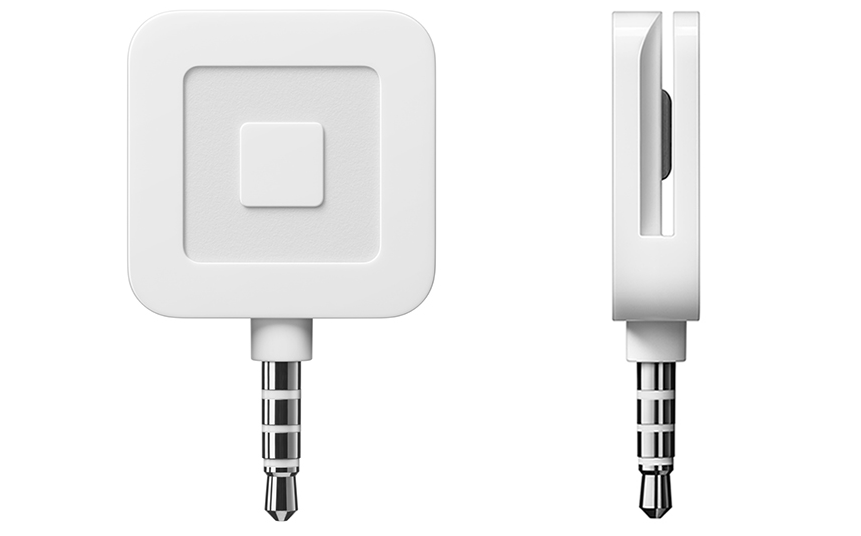
\includegraphics[scale=0.2]{assets/square_reader2.png}\\
  一部の古いクレジットカードでSquareで読み取れない場合はこれを用いる。
  \item iPad\\
  決済を行うのに用いる。
 \end{itemize}
 \subsubsection{使い方}
 \begin{itemize}
  \item クレジットカード
  \begin{itemize}
  \item ICカード
  \begin{enumerate}[手順1]
   \item Square リーダー上部にあるカードスロットに、ICカードのオモテ面を上にしてICチップのある側からカードを挿入する。\\
   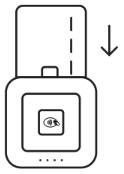
\includegraphics[scale=0.4]{assets/square_insert-card.png}
   \item カードは差し込んだままにし、 Square リーダーから「ピー」と音が鳴って、\\緑色のランプが4つ{\color{green}●●●●}点灯したらカードを取り出す。
   \item お客様にiPadの画面に指でサインをもらい決済を完了する。
  \end{enumerate}
  \item 磁気テープカード\\
  リーダーをiPadのイヤホンジャックに差し込み、磁気テープのみのクレジットカードをスワイプする。
  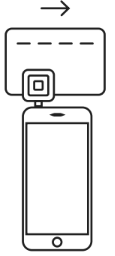
\includegraphics[scale=0.4]{assets/square_slide-card.png}
  \end{itemize}
  \item 電子マネー\\
  交通系IC、QUICPay、iDでの決済
  \begin{enumerate}[手順1]
   \item 「電子マネー」をタップ。
   \item お客様が希望する決済方法を選択。
   \item 青色のランプが4つ{\color{blue} ●●●●}点滅し、画面が「お待ちください。準備をしています。」から「交通系ICカード/iD/QUICPayカードをSquare リーダーにタッチしてください。決済音が鳴るまで動かさないでください。」に変わる。お客様に支払い金額を確認いただき、カードもしくはモバイル端末をSquare リーダーにタッチしてもらう。
   \item POSレジから「ピピッ」と決済音が鳴ったら決済完了。
  \end{enumerate}
 \end{itemize}

\subsection{展示団体入退場管理システム}
\subsection{入場システム}
\subsection{外務送付状の差込}\label{sec:外務送付状の差込}
\section{体育祭}
\subsection{名簿管理}
\subsection{Tシャツ}
\subsection{装飾物デザイン}
\subsection{オンライン得点板}
\subsection{撮影}
\subsection{動画局}


\section{生徒会}

\section{さいごに}

\section{APPENDIX}
\subsection{Githubの使い方}
\subsection{技術局名簿}
\end{document}
